\documentclass[a4paper,ngerman,11pt,bibliography=totoc]{scrartcl}


\usepackage[utf8]{inputenc}

\usepackage[ngerman]{babel}

\usepackage{amsmath, amsthm, amssymb, stmaryrd, color, graphicx, mathtools, mathrsfs}
\usepackage{setspace}
\usepackage{bussproofs}
\usepackage{array}
\usepackage{booktabs}
\usepackage{comment}
\usepackage{textcomp}
\usepackage{stmaryrd}

\usepackage{tikz}
\usetikzlibrary{shapes,arrows}
% Für kommutative Diagramme
\usepackage{tikz-cd}
% Vermeidet Konflikte mit babel ngerman (speziell bei Verwendung der \arrowvert[r, "Text"]-Notation)
\usetikzlibrary{babel}

\usepackage[protrusion=true,expansion=true]{microtype}

\usepackage{lmodern}
\usepackage{tabto}

\usepackage[backend=bibtex,style=alphabetic]{biblatex}
\usepackage[babel]{csquotes}
\bibliography{literatur}

% sidewaystable
\usepackage{rotating}

\usepackage{titling}

\usepackage[all]{xy}

% Automatische Referenzen mit Namen
\usepackage[colorlinks=true, linkcolor=blue, urlcolor=blue, citecolor=blue]{hyperref}
\usepackage{cleveref}			% Referenzen mit Name

\usepackage{icomma}				% Korrektes Typesetting von Kommazahlen

\usepackage[font={small,it}]{caption} % Kleinere Captions

% Für \Set{ ... | ... }
\usepackage{braket}
% Für fette Symbole in Math-Umgebung (\bm)
\usepackage{bm}


%\usepackage{algorithm}
%\usepackage{algpseudocode}
%\algrenewcommand{\algorithmiccomment}[1]{\hskip3em$\slash\slash$ #1}
%\newcommand{\LineFor}[2]{\State\algorithmicfor\ {#1}\ \algorithmicdo\ {#2} \algorithmicend\ \algorithmicfor}
%
%\usepackage{listings}			% Anzeige von Sourcecode

\setlength\parskip{\medskipamount}
\setlength\parindent{0pt}

\theoremstyle{definition}
\newtheorem{defn}{Definition}[section]
\newtheorem{axiom}[defn]{Axiom}
\newtheorem{bsp}[defn]{Beispiel}

\theoremstyle{plain}

\newtheorem{prop}[defn]{Proposition}
\newtheorem{lemma}[defn]{Lemma}
\newtheorem{kor}[defn]{Korollar}
\newtheorem{satz}[defn]{Satz}

\theoremstyle{remark}
\newtheorem{erin}[defn]{Erinnerung}
\newtheorem{bem}[defn]{Bemerkung}
\newtheorem{beob}[defn]{Beobachtung}
\newtheorem{notation}[defn]{Notation}

\clubpenalty=10000
\widowpenalty=10000
\displaywidowpenalty=10000

\newcommand{\IZ}{\mathbb{Z}}
\newcommand{\IQ}{\mathbb{Q}}
\newcommand{\IR}{\mathbb{R}}
\newcommand{\IC}{\mathbb{C}}
\newcommand{\IN}{\mathbb{N}}
\newcommand{\INo}{\IN_0}
\newcommand{\INs}{\IN^\ast}
\newcommand{\Ic}{\mathcal{I}}
\newcommand{\Jc}{\mathcal{J}}
\newcommand{\Hc}{\mathcal{H}}
\newcommand{\Tc}{\mathcal{T}}
\newcommand{\Sc}{\mathcal{S}}
\newcommand{\Oc}{\mathcal{O}}
\newcommand{\Pc}{\mathcal{P}}

\newcommand{\PSet}{\Pc}		% Potenzmenge

\newcommand{\ceil}[1]{\left\lceil#1\right\rceil}
\newcommand{\abs}[1]{\left|#1\right|}

\newcommand{\id}{\mathrm{id}}

\newcommand{\setMid}{\,\middle|\,}

% Supresses qed-symbol in current environment
\newcommand{\noqed}{\let\qed\relax}

\newcommand{\symDiff}{\triangle}


%draft-options:
\definecolor{darkgreen}{rgb}{0,0.6,0.35}
\usepackage[ngerman, textsize=small, textwidth=4.5cm, color=darkgreen]{todonotes}
\usepackage[left=1cm, right=5cm]{geometry}


% Nur für dieses Dokument %%%%%%%%%%%%%%%%%%%%%%%%%%%%%%%%%%%%%%

\setcounter{tocdepth}{3}


\usepackage{tabu}
\usepackage{tabularx}


\newcommand{\dIff}{\mathbin{~\mathop:\!\!\iff}}

% Ordnungsrelation auf dem Kostenraum
\newcommand{\cordleq}{\preccurlyeq}
\newcommand{\cordgeq}{\succcurlyeq}
\newcommand{\cordle}{\prec}
\newcommand{\cordge}{\succ}

\newcommand{\PfadAend}{\delta}
\newcommand{\invPf}[1]{\overset{\leftarrow}{#1}}
\newcommand{\Pfadkomp}{\cdot}

\newcommand{\SVord}{\ensuremath \prec_\uparrow}
\newcommand{\NVrel}{\approx}
\newcommand{\XmodNV}{X/{\NVrel}}
\newcommand{\VerbRel}{\ensuremath <_\uparrow}
\newcommand{\BAord}{\ensuremath \prec^\ast}
\newcommand{\BArel}{\approx^\ast}
\newcommand{\XmodBA}{X/{\BArel}}

% Sammelbegriff für alle Potentialbegriffe
\newcommand{\sPot}{\_-Potential}

% Für Spiele
\newcommand{\Epsilon}{\mathrm{E}}

% DOCUMENT %%%%%%%%%%%%%%%%%%%%%%%%%%%%%%%%%%%%%%%%%%%%%%%%%%%%%

\begin{document}
	
% Spezielle Silbentrennung:
\hyphenation{Ko-or-di-na-tion Ko-or-di-na-tions-spie-len Ko-or-di-na-tions-spiels Be-o-bach-tung}	
	
	
% Titelseite:

\author{Lukas Graf}
\date{Letzte Aktualisierung: \today}

\selectlanguage{ngerman}
\thispagestyle{empty}


\begin{titlepage}\center
	\textsc{\LARGE Universität Augsburg}\\[1cm]
	
	\textsc{\Large Institut für Mathematik}\\[1.5cm]
	
	% Title
	{\Large Masterarbeit \\[1cm]}
	{\huge \todo[inline]{Insert Title}}

	\vfill
	
	% Author and supervisor
	\begin{minipage}{0.4\textwidth}
		\begin{flushleft} \large
			\emph{von:}\\
			Lukas \textsc{Graf}
		\end{flushleft}
	\end{minipage}
	\begin{minipage}{0.4\textwidth}
		\begin{flushright} \large
			\emph{Betreut von:} \\
			Prof. Dr. Tobias \textsc{Harks}
		\end{flushright}
	\end{minipage}
	
\end{titlepage}

% CONTENT %%%%%%%%%%%%%%%%%%%%%%%%%%%%%%%%%%%%%%%%%%%

\tableofcontents

\listoftodos

\newpage
\phantomsection
\addcontentsline{toc}{section}{Einleitung}
\section*{Einleitung}

\todo[inline]{Einleitung schreiben}

Satz von \citeauthor{MonShap}.

\todo[inline,nolist]{Überblick:}

Nachdem wir in \Cref{sec:Grundlagen} einige Grundbegriffe der Spieltheorie definiert haben, werden wir uns zunächst in \Cref{sec:Potentiale} dem Konzept der Potentialfunktionen für Spiele zuwenden. Wir werden eine ganze Reihe derartiger Potentiale kennenlernen und jeweils notwendige und hinreichende Bedingungen dafür zeigen, dass ein Spiel ein entsprechendes Potential besitzt.


\todo[inline,nolist]{Morphismen-Kapitel}

Diese Morphismen werden wir schließlich in \Cref{sec:Auslastungsspiele} nutzen um verschiedene Beziehungen zwischen unterschiedlichen Klassen von Auslastungs- und Potentialspielen zu formulieren und zu zeigen.


\section{Grundlagen}\label{sec:Grundlagen}

\begin{defn}
	Ein \emph{Spiel $\Gamma$ in strategischer Form} ist ein Tupel $(I, X = (X_i)_{i \in I}, (K_i)_{i\in I}, (c_i)_{i\in I})$. Dabei ist
	\begin{itemize}
		\item $I$ die Menge der Spieler,
		\item $X_i$ die Menge der (reinen) Strategien von Spieler $i$,
		\item $(K_i, \cordleq)$, eine total geordnete Menge, der Kostenraum von Spieler $i$ und
		\item $c_i: X_i \to K_i$ die Kostenfunktion von Spieler $i$.
	\end{itemize}
	Das eigentliche Spiel besteht nun daraus, dass jeder Spieler versucht durch die Wahl seiner Strategie die eigenen Kosten zu minimieren.
	
	wir nennen ein solches Spiel \emph{endlich}, wenn der gesamte Strategieraum $X$ endlich ist.
\end{defn}

\begin{beob}
	Klassische Kostenminimierungsspiele erhält man durch Wahl von $(\IR_{\geq 0}, \leq)$ als Kostenraum für alle Spieler, Nutzenmaximierungsspiele durch Wahl von $(\IR, \geq)$ als \glqq Kosten\grqq raum.
\end{beob}

\begin{beob}
	Ist ein Spiel endlich, so können wir in der Regel ohne Einschränkung annehmen, dass auch die Menge der Spieler endlich ist. Denn die Menge $X = \prod_{i\in I} X_i$ kann nur endlich sein, wenn höchsten endliche viele $X_i$ einelementig sind. Also haben in einem endlichen Spiel nur endlich viele Spieler mehr als eine Strategie. Für die Suche beispielsweise nach Nash-Gleichgewichten oder Verbesserungspfaden spielen aber nur solche Spieler eine Rolle. \todo{Kann man diese Erkenntnis irgendwie mit Morphismen formalisieren (evtl. über Retrakte?)}
\end{beob}

\begin{notation}
	Zu einem festen Spieler $i$ bezeichne $X_{-i} := \prod_{j \in I\backslash\{i\}} X_j$ das Produkt aller Strategieräume außer dem von Spieler $i$. Zu jedem Strategieprofil\todo{Sollte der Begriff Strategieprofil eigens definiert werden?}{} $x \in X$ bezeichne dann $x_{-i}$ die Projektion dieses Profils auf den Raum $X_{-i}$ und $x_i$ die Projektion auf $X_i$ (also die von Spieler $i$ gewählte Strategie). Wir schreiben dann auch $(x_i, x_{-i})$ für das Strategieprofil $x$.
	
	Später werden wir auch Abbildungen $\phi_i: X_i \to Y_i$ zwischen den spielerspezifischen Strategieräumen betrachten und die durch diese induzierte Abbildung $X \to Y: x = (x_i)_{i \in I} \mapsto \phi(x) := (\phi_i(x_i))_{i \in I}$ mit $\phi$ bezeichnen. Analog zur Notation für Strategieräume werden wir außerdem die Notation $\phi_{-i}: X_{-i} \to Y_{-i}$ verwenden.
\end{notation}

\begin{defn}
	Ein Strategieprofil $x \in X$ ist ein \emph{Nash-Gleichgewicht}, wenn für jeden Spieler $i \in I$ und jede seiner Strategien $\hat{x}_i$ gilt:
		\[c_i(\hat{x}_i, x_{-i}) \cordgeq c_i(x)\]
	Ein Nash-Gleichgewicht ist also ein Strategieprofil, aus dem heraus kein Spieler einen Anreiz für einen einseitigen Strategiewechsel hat.	
\end{defn}

Aus \cite{MonShap}:

\begin{defn}
	Eine Folge von Strategieprofilen $x^0, x^1, x^2, \dots$ ist ein \emph{Verbesserungspfad}, wenn folgende beiden Eigenschaften erfüllt sind:
	\begin{enumerate}
		\item Für jede Stelle $n$ gibt es einen Spieler $i(n) \in I$, sodass das Profil $x^{n+1}$ aus $x^n$ durch alleinige Abweichung dieses Spielers entsteht, d.h. $x^{n+1} = (x^{n+1}_{i(n)}, x^n_{-i(n)})$
		\item Der abweichende Spieler $i(n)$ verbessert sich, d.h. $c_{i(n)}(x^{n+1}) \cordle c_{i(n)}(x^n)$.
	\end{enumerate}
	Wir nennen einen endlichen Verbesserungspfad $x^0, x^1, \dots, x^n$ \emph{abgeschlossen}, wenn er nicht mehr nach hinten verlängert werden kann, d.h. es keine Strategie $\hat{x}_i$ gibt, mit $c_{i}(x^n_{-i}, \hat{x}_i) \cordle c_{i}(x^n)$.
\end{defn}

\begin{defn}
	Ein Spiel $\Gamma$ hat die \emph{finite improvement property (FIP)}, wenn jeder Verbesserungspfad endlich ist.
\end{defn}

\begin{beob}\label{beob:VerbPfadeundNGe}
	Jedes Ende eines abgeschlossenen Verbesserungspfades ist ein Nash-Gleichgewicht. Denn wäre dem nicht so, dann gäbe es wenigstens einen Spieler, der sich durch Abweichen noch verbessern kann - was zu einer Verlängerung des Verbesserungspfades führen würde. 
		
	Umgekehrt ist offenkundig auch jedes Nash-Gleichgewicht Ende wenigstens eines abgeschlossenen Verbesserungspfades - nämlich des trivialen, nur aus diesem Strategieprofil bestehenden Verbesserungspfades
\end{beob}

\begin{kor}\label{kor:ExVerbPfadExNG}\todo{Sollte eine Beobachtung wirklich ein Korrolar haben?}
	Ein Spiel $\Gamma$ besitzt genau dann (mindestens) ein Nash-Gleichgewicht, wenn es (mindestens) einen endlichen, maximalen Verbesserungspfad besitzt. Ein Spiel mit FIP besitzt dementsprechend immer wenigstens ein Nash-Gleichgewicht.
\end{kor}

Aus \cite{BestRespPot}

\begin{defn}
	Ein Verbesserungspfad $x^0, x^1, x^2, \dots$ heißt \emph{Beste Antwort-Pfad}\todo{Voorneveld nennt es (ohne Verbesserungsbedinung) beste Antwort-kompatibel}, wenn der abweichende Spieler jeweils eine beste Alternativstrategie wählt, d.h. 
		\[c_{i(n)}(x^{n+1}) = \min_{\hat{x}_{i(n)} \in X_{i(n)}} c_{i(n)}(\hat{x}_i,x^n_{-i(n)}).\]
	\todo{Insbesondere setzt das natürlich voraus, dass ein solches Maximum auf dem Pfad immer existiert.}
\end{defn}

\section{Potentiale}\label{sec:Potentiale}

Eine Schwierigkeit bei der Analyse von Spielen bildet der Umstand, dass jeder Spieler eine eigene Kostenfunktion und damit ein eigenes Optimierungsziel hat. Möchte man also beispielsweise Gleichgewichtspunkte finden, so muss man alle diese Funktionen gleichzeitig (lokal) optimieren. Diese Aufgabe wird wesentlich einfacher, wenn das Spiel eine sogenannte \emph{Potentialfunktion} besitzt. Das ist eine Funktion auf dem Strategieraum des Spieles, die ein alternatives Koordinationsspiel darauf definiert, welches gewisse Eigenschaften mit dem ursprünglichen Spiel teilt (etwa die Lage der Gleichgewichtspunkte).

In diesem Kapitel werden wir einige Varianten von Potentialfunktionen kennenlernen und feststellen, welche Spiele diese jeweils besitzen. In \Cref{sec:Morphismen} werden wir dann die Beziehung zwischen Ausgangsspiel und dem von einer Potentialfunktion beschriebenen Koordinationsspiel durch Morphismen zwischen den beiden Spielen formalisieren und dadurch zeigen, welche Eigenschaften beim Wechsel zwischen den beiden Spielen erhalten bleiben.

\subsection{Definitionen}

Zunächst definieren wir eine Auswahl verschiedener Typen von Potentialfunktionen:

\begin{defn}
	Zu einem Spiel $\Gamma = (I, X, (c_i))$ heißt eine Funktion $P: X \to \IR$
	\begin{itemize}
		\item \emph{verallgemeinertes Nash-Potential}, wenn jedes Minimum von $P$ ein Nash-Gleichgewicht in $\Gamma$ ist, d.h. für alle $x \in X$ gilt:
			\[P(x) = \min_{\hat{x} \in X}P(\hat{x}) \implies \forall i \in I, \hat{x}_i \in X_i: c_i(x) \leq c_i(x \mid \hat{x}_i) \]
		\item \emph{Nash-Potential}, wenn jedes Minimum von $P$ ein Nash-Gleichgewicht in $\Gamma$ ist und umgekehrt, d.h. für alle $x \in X$ gilt:
			\[P(x) = \min_{\hat{x} \in X}P(\hat{x}) \iff \forall i \in I, \hat{x}_i \in X_i: c_i(x) \leq c_i(x \mid \hat{x}_i) \]
		\item \emph{lokales Nash-Potential}, wenn jedes \glqq lokale\grqq{} Minimum von $P$ ein Nash-Gleichgewicht in $\Gamma$ ist und umgekehrt, d.h. für alle $x \in X$ gilt:
			\[\forall i \in I, \hat{x}_i \in X_i: P(x) \leq P(x \mid \hat{x}_i) \iff \forall i \in I, \hat{x}_i \in X_i: c_i(x) \leq c_i(x \mid \hat{x}_i) \]
		\item \emph{Beste-Antwort-Potential}, wenn für jeden Spieler $i$ und alle Strategieprofile $x \in X$ gilt:
			\[\arg\min_{\hat{x}_i \in X_i}c_i(x \mid \hat{x}_i) = \arg \min_{\hat{x}_i \in X_i} P(x \mid \hat{x}_i)\]
		\item \emph{verallgemeinertes ordinales Potential}, wenn für jeden Spieler $i$ und alle Strategieprofile $x \in X$ sowie $\hat{x}_i \in X_i$ gilt:
			\[c_i(x) > c_i(x \mid \hat{x}_i) \implies P(x) > P(x \mid \hat{x}_i)\]
		\item \emph{ordinales Potential}, wenn für jeden Spieler $i$ und alle Strategieprofile $x \in X$ sowie $\hat{x}_i \in X_i$ gilt:
			\[c_i(x) > c_i(x \mid \hat{x}_i) \iff P(x) > P(x \mid \hat{x}_i)\]
		\item \emph{skaliertes Potential}, wenn es streng monotone Funktionen $f_i: \IR \to \IR$ gibt, sodass für jeden Spieler $i$ und alle Strategieprofile $x \in X$ sowie $\hat{x}_i \in X_i$ gilt:
			\[c_i(x) - c_i(x \mid \hat{x}_i) = f_i(P(x)) - f_i(P(x \mid \hat{x}_i))\]
		\item \emph{gewichtetes Potential}, wenn es einen Gewichtsvektor $(w_i)_{i\in I} \in \IR_{>0}^I$ gibt, sodass für jeden Spieler $i$ und alle Strategieprofile $x \in X$ sowie $\hat{x}_i \in X_i$ gilt:
			\[c_i(x) - c_i(x \mid \hat{x}_i) = w_i\cdot(P(x) - P(x \mid \hat{x}_i))\]
		\item \emph{exaktes Potential}, wenn für jeden Spieler $i$ und alle Strategieprofile $x \in X$ sowie $\hat{x}_i \in X_i$ gilt:
			\[c_i(x) - c_i(x \mid \hat{x}_i) = P(x) - P(x \mid \hat{x}_i)\]
	\end{itemize}
\end{defn}

Exakte, gewichtete, ordinale und verallgemeinerte ordinale Potentiale wurden erstmals in \cite{MonShap} definiert, beste Antwort-Potentiale erstmals in \cite{BestRespPot}. Die Begriffe verallgemeinertes und lokales Nash-Potential dürften für die Anwendung eher weniger interessant sein, sondern sollen vor allem das grundlegende Konzept eines Potentials formalisieren und umfassen daher auch (fast) alle anderen Potentiale. Die Beziehungen zwischen den verschiedenen Potentialbegriffen werden in dem an \cite[Abbildung 1]{BestRespPot} angelehnten Euler-Diagramm (\Cref{diag:Potentiale}) dargestellt.

\begin{figure}[h]\centering
	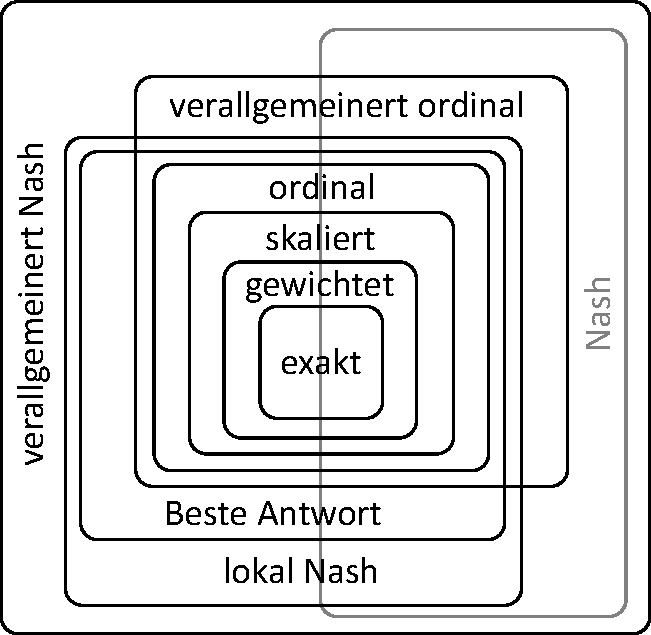
\includegraphics[width=.4\textwidth]{../Bilder/EulerDiagPotentiale.pdf}
	\caption{Beziehungen zwischen den einzelnen Potentialbegriffen}\label{diag:Potentiale}
\end{figure}

\begin{bsp}
	Jedes Koordinationsspiel besitzt ein exaktes Potential (nämlich die gemeinsame Kostenfunktion). Ebenso besitzt jedes Dummyspiel ein exaktes Potential (nämlich die konstante $0$-Funktion).
	
	Entsprechend besitzt jedes skalierte Koordinationsspiel ein skaliertes Potential.
\end{bsp}

\subsection{Anschauung}

Verallgemeinerte Nash-Potentiale (und damit alle oben beschriebenen Potentiale) formalisieren die Idee ein Spiel durch irgendein anderes mit einer einzigen Funktion beschriebenes Optimierungsproblem zu ersetzen, dessen Optima Nash-Gleichgewichte im ursprünglichen Spiel sind. Im Falle eines Nash-Potentials entsprechen diese Optima sogar allen Nash-Gleichgewichten. Findet man nun ein solches Optimierungsproblem und kann von diesem zeigen, dass es immer ein Optimum besitzt (etwa weil es durch eine stetige Funktion beschrieben wird und der Strategieraum kompakt ist), so zeigt dies, dass das ursprüngliche Spiel mindestens ein Nash-Gleichgewicht besitzt. Außerdem kann man dieses durch Lösen des Optimierungsproblems bestimmen.

Versteht man zu einem gegebenen Strategieprofil $x \in X$ dessen \emph{Nachbarschaft} als die Menge aller durch höchstens einen Schritt erreichbarer Strategieprofile, d.h. die Menge $\set{(x \mid \hat{x}_i) | i \in I, \hat{x}_i \in X_i}$, so nennen wir $x$ ein \emph{lokales Minimum} einer Funktion $P: X \to \IR$, wenn es ein Minimum innerhalb seiner Nachbarschaft ist. Ein lokales Nash-Potential beschreibt damit ein Optimierungsproblem, dessen \emph{lokale} Minima den Nash-Gleichgewichten des Ausgangsspiels entsprechen.

Die Nachbarschaft eines Strategieprofils $x$ besteht nun gerade aus den Profilen, die man mit $x$ vergleichen muss, um festzustellen, ob es sich bei $x$ um ein Nash-Gleichgewicht handelt. Hat man also ein Spiel $\Gamma = (I, X, (c_i))$ mit einem lokalen Nash-Potential $P$, so induziert dieses ein Koordinationsspiel $\Kappa \coloneqq (I, X, (P))$ auf dem selben Strategieraum, dessen Nash-Gleichgewichte gerade mit denen des Spiels $\Gamma$ übereinstimmen.

Weitere Spezialisierungen dieses Potentialbegriffs führen dann zu induzierten Koordinationsspielen, welche noch mehr Eigenschaften des Ausgansspiels übernehmen: So hat das durch ein Beste-Antwort-Potential beschriebene Spiel etwa die gleichen Beste-Antwort-Pfade und eignet sich daher beispielsweise zur Analyse von Beste-Antwort-Dynamiken. Durch ein ordinales Potential erhält man ein Spiel, welches auch die gleichen Verbesserungs- und Nichtverschlechterungspfade besitzt. Bei einem verallgemeinerten ordinalen Potential bleiben diese hingegen jeweils nur in eine Richtung erhalten: Ein Verbesserungspfad im Ausgangsspiel ist auch einer im Koordinationsspiel und ein Nichtverschlechterungspfad im Koordinationsspiel entspricht einem solchen im ursprünglichen Spiel (vgl. \Cref{prop:ordPotVerbpfad}).

Für skalierte, gewichtete und exakte Potentiale gibt es eine noch anschaulichere Betrachtungsweise für den Fall (endlicher) 2-Personenspiele. Statt als Matrix kann man deren Strategieraum auch als Gitternetz in der Ebene auffassen, wobei jede Strategie von Spieler 1 einer waagerechten und jede Strategie von Spieler 2 einer senkrechten Gitterlinie entspricht. Kreuzungspunkte von zwei Gerade entsprechen dann gerade vollständige Strategieprofilen. Kostenfunktionen (ebenso wie Potentiale) sind dann \glqq Reliefkarten\grqq{}, deren Höhe den jeweiligen Kosten entspricht. 

\begin{figure}[h]\centering
	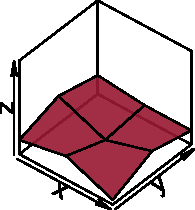
\includegraphics[width=.3\textwidth]{../Bilder/exaktesPotentialSp1.pdf}
	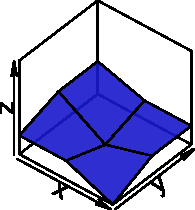
\includegraphics[width=.3\textwidth]{../Bilder/exaktesPotentialSp2.pdf}
	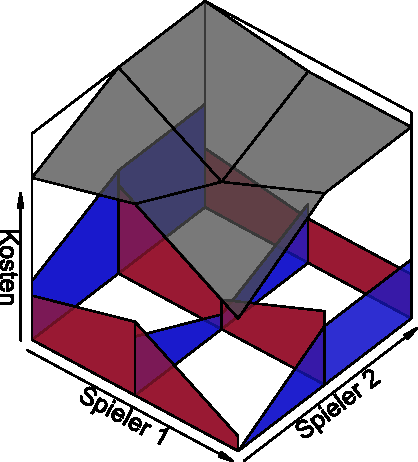
\includegraphics[width=.3\textwidth]{../Bilder/exaktesPotential.pdf}
	\caption{Ein 2-Personenspiel mit exaktem Potential (grau): Spieler 1: rot, Spieler 2: blau}
\end{figure}

Ein Potential entspricht in diesem Bild einer gemeinsamen Reliefkarte für beide Spieler, die - im Falle eines exakten Potentials - \glqq scheibenweise\grqq{} bis auf eine additive Konstante mit der eigentlichen Kostenfunktion übereinstimmt. Anders formuliert: Wird die Strategie eines Spieler festgehalten, so kann der andere Spieler seine Kostenveränderungen bei der Wahl der verschiedenen ihm zur Verfügung stehenden Strategien auch anhand der Potentialfunktion ablesen. 

Geht man nun über zu einem skalierten Potential, so lesen die beiden Spieler das Potential sozusagen in verschiedenen Einheiten ab (müssen das Potential also erst noch passend skalieren um ihre tatsächliche Veränderung zu bekommen). Sind die Skalierungsfunktionen linear (das Potential also sogar ein gewichtetes), dann sind die verschiedenen Einheiten proportional zueinander.


\subsection{Eigenschaften der Potentiale}

Wir wollen hier noch einige Eigenschaften der verschiedenen Potentiale zusammenfassen - beweisen werden wir sie dann aber erst in \Cref{sec:Morphismen}.

\begin{satz}\label{satz:ZusammenaengePotentiale}
	Es gelten die in \Cref{diag:Potentiale} dargestellten Zusammenhänge zwischen den verschiedenen Potentialen.
\end{satz}

Die Zusammenhänge lassen sich alle leicht direkt beweisen. Wir werden diese Beweise hier allerdings nicht führen, da sich die Aussagen auch aus den allgemeineren Sätzen über die entsprechenden Morphismen ergeben, die wir in \Cref{sec:Morphismen} definieren werden (die Beweise finden sich dann in \Cref{sec:Morphismen:Potentialsaetze}). Dass die unterschiedlichen Potentiale auch tatsächlich echt verschiedene Klassen von Spielen beschreiben, zeigen die folgenden Beispiele: 

\begin{bsp}\label{bsp:PotentialInklusionen}
	Es sei jeweils $\gamma \coloneqq ((t,l), (t,r), (b,r), (b,l))$ der $4$-Zykel, der den Strategieraum im Uhrzeigersinn durchläuft. Zum Beweis, dass ein Spiel kein bestimmtes Potential besitzen kann, verwenden wir zum Teil bereits die entsprechenden Charakterisierungen aus \Cref{sec:Potentiale:Charakterisierungen}.
	\begin{itemize}
		\item $\Gamma_1$ besitzt ein gewichtetes, aber kein exaktes Potential:
			\begin{center}
				$\Gamma_1:$ \quad
				\begin{tabular}{c||c|c}
					& l 		& r 		\\\hline\hline
					t	& $(0,0)$	& $(0,0)$	\\\hline
					b	& $(0,0)$	& $(1,2)$ 
				\end{tabular}\hspace{5em}
				$P_1:$ \quad
				\begin{tabular}{c||c|c}
					& l 		& r 		\\\hline\hline
					t	& $0$	& $0$	\\\hline
					b	& $0$	& $1$ 
				\end{tabular}
			\end{center}
			$P_1$ ist ein gewichtetes Potential (mit Gewichtsvektor $(1,2)$), aber $\Gamma_1$ kann nach \Cref{satz:CharExPot} kein exaktes Potential besitzen, da $\PfadAend(\gamma) = 0 + 1 - 2 + 0 \neq 0$ gilt.
		
		\item $\Gamma_2$ besitzt ein skaliertes, aber kein gewichtetes Potential:
			\begin{center}
				$\Gamma_2:$ \quad
				\begin{tabular}{c||c|c}
					& l 		& r 		\\\hline\hline
					t	& $(0,0)$	& $(0,1)$	\\\hline
					b	& $(1,0)$	& $(2,1)$ 
				\end{tabular}\hspace{5em}
				$P_2:$ \quad
				\begin{tabular}{c||c|c}
					& l 		& r 		\\\hline\hline
					t	& $0$	& $1$	\\\hline
					b	& $1$	& $2$ 
				\end{tabular}
			\end{center}
			$P_2$ ist ein skaliertes Potential (mit den Skalierungsfunktionen $f_1(0) \coloneqq 0, f_1(1) = 1, f_1(2) = 3$ und $f_2 \coloneqq \id$). $\Gamma_2$ kann aber kein gewichtetes Potential besitzen. Denn gäbe es ein solches und wäre $w = (w_1, w_2)$ der zugehörige Gewichtsvektor, so würde nach \Cref{satz:CharGewPot} gelten:
				\[0 = \PfadAend_w(\gamma) = w_2(1-0) + w_1(2-0) + w_2(0-1) + w_1(0-1) = w_1 \]
			Das aber wäre ein Widerspruch dazu, dass Gewichtsvektoren positiv sein müssen.
			
		\item $\Gamma_3$ besitzt ein ordinales, aber kein skaliertes Potential:
			\begin{center}
				$\Gamma_3:$ \quad
				\begin{tabular}{c||c|c}
					& l 		& r 		\\\hline\hline
					t	& $(0,0)$	& $(0,0)$	\\\hline
					b	& $(1,0)$	& $(2,0)$ 
				\end{tabular}\hspace{5em}
				$P_3:$ \quad
				\begin{tabular}{c||c|c}
					& l 		& r 		\\\hline\hline
					t	& $0$	& $0$	\\\hline
					b	& $1$	& $1$ 
				\end{tabular}
			\end{center}
			$P_3$ ist ein ordinales Potential, $\Gamma_3$ besitzt aber kein skaliertes Potential. Denn wäre $P$ ein solches skaliertes Potential, dann müsste wegen der strengen Monotonie der Skalierungsfunktion $f_2$ gelten:
				\[P(t,l) = P(t,r) \text{ und } P(b,l) = P(b,r)\]
			Daraus ergäbe sich dann aber der folgende Widerspruch:
				\begin{align*}
					1 = c_1(b,l)-c_1(t,l) 	&= f_1(P(b,l)) - f_1(P(t,l)) = \\
											&= f_1(P(b,r)) - f_1(P(t,r)) = c_1(b,r) - c_1(t,r) = 2
				\end{align*}
	\end{itemize}
	Die folgenden drei Beispiele sind \cite[Beispiele 4.1, 4.2 und 4.3]{BestRespPot} entnommen:
	\begin{itemize}
		\item $\Gamma_4$ besitzt ein verallgemeinert ordinales und ein Beste-Antwort-Potential, aber kein ordinales Potential:
			\begin{center}
				$\Gamma_4:$ \quad
				\begin{tabular}{c||c|c|c}
						& l 		& m			& r 		\\\hline\hline
					t	& $(1,2)$	& $(2,0)$ 	& $(2,1)$	\\\hline
					b	& $(2,2)$	& $(2,0)$	& $(1,2)$
				\end{tabular}\hspace{5em}
				$P_4:$ \quad
				\begin{tabular}{c||c|c|c}
						& l 		& m 		& r \\\hline\hline
					t	& $3$	& $0$ 		& $2$	\\\hline
					b	& $4$	& $0$		& $1$
				\end{tabular}
			\end{center}
			$P_4$ ist sowohl ein verallgemeinertes ordinales als auch ein Beste-Antwort-Potential für $\Gamma_4$, ein ordinales Potential kann es allerdings nach \Cref{satz:CharOrdPot} nicht geben, da $\gamma$ ein schwacher Verbesserungszykel ist.
		\item $\Gamma_5$ besitzt ein verallgemeinertes ordinales Potential, aber kein Beste-Antwort-Potential:
			\begin{center}
				$\Gamma_5:$ \quad
				\begin{tabular}{c||c|c}
						& l 		& r 		\\\hline\hline
					t	& $(1,1)$	& $(1,0)$	\\\hline
					b	& $(1,0)$	& $(0,1)$ 
				\end{tabular}\hspace{5em}
				$P_5:$ \quad
				\begin{tabular}{c||c|c}
						& l 		& r 		\\\hline\hline
					t	& $3$	& $2$			\\\hline
					b	& $0$	& $1$ 
				\end{tabular}
			\end{center}
		$P_5$ ist ein verallgemeinertes ordinales Potential für $\Gamma_5$. Ein Beste-Antwort-Potential hierzu kann es aber nach \Cref{satz:CharExBAPot} nicht geben, da $\gamma$ ein schwacher Beste-Antwort-Verbesserungszykel ist.
		\item $\Gamma_6$ besitzt ein Beste-Antwort-Potential, aber kein verallgemeinertes ordinales Potential:
			\begin{center}
				$\Gamma_6:$ \quad
				\begin{tabular}{c||c|c|c}
						& l 		& m			& r 		\\\hline\hline
					t	& $(1,2)$	& $(0,0)$	& $(2,1)$	\\\hline
					b	& $(2,1)$	& $(2,2)$ 	& $(1,2)$
				\end{tabular}\hspace{5em}
				$P_6:$ \quad
				\begin{tabular}{c||c|c|c}
						& l 		& m 		& r \\\hline\hline
					t	& $1$	& $0$		& $4$	\\\hline
					b	& $2$	& $4$ 		& $3$
				\end{tabular}
			\end{center}
			$P_6$ ist ein Beste-Antwort-Potential zu $\Gamma_6$, ein verallgemeinertes ordinales Potential kann es hingegen laut \Cref{kor:CharExVerOrdPotabzX} nicht geben, da $\gamma$ ein Verbesserungszykel ist.
	\end{itemize}
\end{bsp}

Direkt aus der Definition ergibt sich die folgende Beobachtung über lokale Nash-Potentiale:

\begin{beob}\label{beob:lokMinNG}
	Ist $\Gamma$ ein Spiel mit einem lokalen Nash-Potential $P$. Dann ist jedes lokale Minimum von $P$ ein Nash-Gleichgewicht von $\Gamma$ und umgekehrt.
\end{beob}

Wir können also Nash-Gleichgewichte allein durch Betrachten einer Potentialfunktion finden. Daraus folgt direkt die Existenz von Nash-Gleichgewichten in einer Vielzahl von Potentialspielen, nämlich all diejenigen deren Potentialfunktion mindestens ein globales (und damit erst recht lokales) Minimum haben. Beispielsweise also:

\begin{kor}
	Sei $\Gamma$ ein Spiel mit einem kompakten Strategieraum und einem stetigen verallgemeinerten Nash-Potential. Dann hat $\Gamma$ wenigstens ein Nash-Gleichgewicht.
\end{kor}

Insbesondere haben endliche Potentialspiele immer ein Nash-Gleichgewicht. Wie bereits erwähnt bewahren ordinale Potentiale zudem auch Verbesserungspfade:

\begin{satz}\label{prop:ordPotVerbpfad}
	Sei $\Gamma$ ein Spiel mit einem verallgemeinerten ordinalen Potential $P$. Dann ist jeder Verbesserungspfad in $\Gamma$ auch ein Verbesserungspfad bezüglich $P$. Ist $P$ sogar ein ordinales Potential, so gilt auch die umgekehrte Richtung.
\end{satz}

Analog zu diesem Satz gilt für Beste-Antwort-Pfade und Beste-Antwort-Potentiale:

\begin{satz}\label{prop:BAPotBAPfad}
	Sei $\Gamma$ ein Spiel mit einem Beste-Antwort-Potential $P$. Dann ist jeder Beste-Antwort-(Verbesserungs-)Pfad in $\Gamma$ auch ein Beste-Antwort-(Verbesserungs-)Pfad bezüglich $P$ und umgekehrt.
\end{satz}

\Cref{tab:PotErhalten} fasst einige der von Potentialen erhaltenen Eigenschaften zusammen.

\begin{table}[h]\centering
	\begin{tabular}{l|ccccc}
						& Nash-Gl. 			& FIP 					& Nichtverschl.pfad 			& Verb.pfad 		& Beste-Antwort-Pfad \\\hline
		exakt			& $\Leftrightarrow$	& $\Leftrightarrow$ 	& $\Leftrightarrow$				& $\Leftrightarrow$	& $\Leftrightarrow$ \\
		gewichtet		& $\Leftrightarrow$	& $\Leftrightarrow$ 	& $\Leftrightarrow$				& $\Leftrightarrow$	& $\Leftrightarrow$ \\		
		skaliert		& $\Leftrightarrow$ & $\Leftrightarrow$ 	& $\Leftrightarrow$				& $\Leftrightarrow$	& $\Leftrightarrow$ \\
		ordinal			& $\Leftrightarrow$	& $\Leftrightarrow$ 	& $\Leftrightarrow$				& $\Leftrightarrow$	& $\Leftrightarrow$ \\
		verallg. ordinal& $\Leftarrow$		& $\Leftarrow$		 	& $\Leftarrow$					& $\Rightarrow$		& $\Rightarrow$ 	\\
		Beste Antwort	& $\Leftrightarrow$	& 					 	& 								& 					& $\Leftrightarrow$ \\
		lokal Nash		& $\Leftrightarrow$	& 					 	& 								& 					& 					
	\end{tabular}	
	\caption{Welche Eigenschaft bleibt beim Übergang von einem Spiel auf das von einem entsprechenden Potential induzierte Koordinationsspiel erhalten ($\Rightarrow$) und welche bei der umgekehrten Richtung ($\Leftarrow$)?}\label{tab:PotErhalten}
\end{table}

Für Spiele mit unendlicher Spielermenge wird sich im folgenden Abschnitt die Beobachtung als hilfreich erweisen, dass wir die meisten Potentiale pfadzusammenhangskomponentenweise definieren können:

\begin{beob}\label{beob:KompWeisePotentiale}
	Sei $\Gamma$ ein beliebiges Spiel und $P: X \to \IR$ eine Funktion. Erfüllt $P$ dann die Bedingung eines exakten/ordinalen/verallgemeinerten ordinalen/Beste-Antwort/lokalen Nash-Potentials für jede (maximale) Pfadzusammenhangskomponente, so ist $P$ ein entsprechendes Potential für ganz $\Gamma$.
	
	Für gewichtete/skalierte Potentiale gilt die entsprechende Aussage nur mit der Zusatzbedingung, dass die verschiedenen Potentiale auf den Pfadzusammenhangskomponenten jeweils die gleichen Gewichte bzw. Skalierungsfunktionen verwenden.
\end{beob}

\begin{proof}
	Dies folgt direkt aus dem Umstand, dass die definierende Eigenschaft für alle aufgezählten Potentiale immer nur entlang eines Pfades (der Länge $1$) und damit innerhalb einer Zusammenhangskomponente geprüft werden muss.
\end{proof}


\subsection{Charakterisierungen der Potentiale}\label{sec:Potentiale:Charakterisierungen}

In diesem Abschnitt wollen wir für einige der zuvor beschriebenen Potentiale notwendige und hinreichende Anforderungen an ein Spiel finden dafür, dass dieses ein entsprechendes Potential besitzt.

\subsubsection{Exakte Potentiale}

\begin{satz}\label{satz:CharExPot}
	Ein Spiel besitzt genau dann ein exaktes Potential, wenn alle 4-Zykel im Strategieraum eine Gesamtänderung von $0$ haben.
\end{satz}

\begin{proof}
	Wir folgen dem Beweis aus \cite[Anhang A]{MonShap}. Dort wird der Satz zwar nur für $N$-Personenspiele gezeigt, mit \Cref{beob:KompWeisePotentiale} überträgt sich dieser Beweis aber direkt auch auf allgemeine Spiele.
	
	Sei zunächst $\gamma \coloneqq (x^0, x^1, x^2, x^3, x^4)$ ein beliebiger 4-Zykel in einem Spiel mit exaktem Potential $P$. Dann gilt für die Gesamtänderung entlang dieses Pfades:
		\[\PfadAend(\gamma) = \sum_{k=1}^4 \left(c_{i(k)}(x^k) - c_{i(k)}(x^{k-1})\right) = \sum_{k=1}^{4} \left(P(x^k) - P(x^{k-1})\right) = P(x^4) - P(x^0) = 0^{}\]
		
	Ist umgekehrt $\Gamma$ ein Spiel, in dem für alle 4-Zykel $\gamma$ gilt $\PfadAend(\gamma) = 0$, $\hat{x}$ ein beliebiges, aber festes Strategieprofil in $\Gamma$ und $Y_{\hat{x}}$ dessen Pfadzusammenhangskomponente, dann definiere wie folgt eine Funktion $P_{\hat{x}}$ auf $Y_{\hat{x}}$:
		\[P_{\hat{x}}: Y_{\hat{x}} \to \IR: x \mapsto \PfadAend(\gamma), \,\gamma \text{ beliebiger Pfad von } \hat{x} \text{ nach } x \]
	Damit diese Funktion tatsächlich wohldefiniert ist, muss für je zwei Pfade $\gamma_1$ und $\gamma_2$ von $\hat{x}$ nach $x$ gelten, dass die jeweiligen Gesamtänderungen gleich sind, d.h. $\PfadAend(\gamma_1) = \PfadAend(\gamma_2)$. Dies ist nach \Cref{beob:Pfade} äquivalent zu
		\[\PfadAend\left(\gamma_1 \cdot \overset{\leftarrow}{\gamma_2}\right) = 0.\]
	Dazu zeigen wir nun mittels Induktion über deren Länge, dass für alle Zykel $\mu$ gilt $\PfadAend(\mu) = 0$:
	\begin{description}
		\item[IA ($\bm{\abs{\mu}=4}$)]\hspace{-.5em}\footnote{Zykel der Längen $0$, $1$, $2$ und $3$ haben automatisch immer Gesamtänderung $0$, da in ihnen alle Abweichungen vom gleichen Spieler vorgenommen werden müssen.} D.h. $\mu$ ist ein 4-Zykel und damit $\PfadAend(\mu) = 0$ nach Voraussetzung.
		\item[IS ($\bm{\abs{\mu}\eqqcolon n}$)] Vorausgesetzt es gibt einen Pfad $\mu' = (x'^0, \dots, x'^n)$ gleicher Länge und Gesamtänderung wie $\mu$, sodass in den ersten beiden Schritten der gleiche Spieler seine Strategie wechselt, d.h. $i(1)=i(2)$. Dann erhält man durch Weglassen des ersten Schrittes einen \emph{kürzeren} Pfad $\mu'' \coloneqq (x'^0, x'^2, \dots, x'^n)$ mit gleicher Gesamtänderung, welche dann nach Induktion bereits $0$ ist. In diesem Fall haben wir dann wie gewünscht $\PfadAend(\mu) = \PfadAend(\mu') = \PfadAend(\mu'') = 0$.
		
		Die Existenz eines derartigen Pfades $\mu'$ zeigen wir nun mittels Induktion über $k \coloneqq \min\left\{1 < l \leq n \setMid i(l) = i(1)\right\}$. Wenigstens ein solches $k$ existiert immer, da Spieler $i(1)$ bereits im ersten Schritt seine Strategie wechselt und dies daher im Verlauf des Zykels noch mindestens ein weiteres Mal tun muss, damit der Zykel geschlossen werden kann.
		\begin{description}
			\item[IA ($\bm{k=2}$)] Dann gilt bereits $i(1)=i(2)$ und wir sind fertig mit $\mu' \coloneqq \mu$.
			\item[IS ($\bm{k-1\to k}$)] Wir ändern $\mu$ so ab, dass Spieler $i(1)$ schon im $(k-1)$-ten Schritt der abweichende Spieler ist. Dann sind wir fertig nach Induktionsvoraussetzung. Dazu ersetzen wir in $\mu$ das Strategieprofil $x^{k-1}$ durch $(x^{k-2} \mid x^{k}_{i(1)})$, sodass also Spieler $i(1)$ bereits einen Schritt früher (im $(k-1)$-ten) seine Strategie wechselt und der Spieler, der dies zuvor in diesem Schritt getan hat, einen Schritt später.
			
			Bei dieser Anpassung bleibt die Gesamtänderung des Pfades $\mu$ gleich, denn wir ersetzen lediglich ein Pfadstück der Länge $2$ durch ein anderes Pfadstück der Länge $2$. Und da sich diese beiden Pfade zu einem 4-Zykel zusammensetzen lassen, haben diese nach Voraussetzung die gleiche Gesamtänderung.
			
			Auf dieses abgeänderte $\mu$ können wir nun die Induktionsvoraussetzung anwenden und erhalten dadurch einen neuen Pfad $\mu'$ mit den gewünschten Eigenschaften.
		\end{description}
		Hiermit können wir auch den Induktionsschritt der äußeren Induktion und damit den Nachweis der Wohldefiniertheit von $P_{\hat{x}}$ abschließen. 
	\end{description}	
	Wählen wir nun für jede maximale Pfadzusammenhangskomponente ein einziges $\hat{x}$ in dieser und definieren wie oben eine Funktion $P_{\hat{x}}$, so lassen sich alle diese Funktionen zu einer Funktion $P$ auf ganz $X$ zusammensetzen. Nach Definition erfüllt diese auf jeder Pfadzusammenhangskomponente die Bedingung eines exakten Potentials. Also ist $P$ nach \Cref{beob:KompWeisePotentiale} ein exaktes Potential auf $X$.
\end{proof}

Eine alternative Charakterisierung für die Existenz eines exakten Potentials zeigen \citeauthor{KoordDummy} in \cite[Theorem 2.1]{KoordDummy}:

\begin{satz}\label{satz:CharExPotAlt}
	Ein Spiel $\Gamma = (I, X, (c_i))$ besitzt genau dann ein exaktes Potential, wenn es ein Koordinationsspiel $\Kappa = (I, X, (p))$ und ein Dummy-Spiel $\Dummy = (I, X, (d_i))$ auf dem selben Strategieraum gibt, sodass die Kostenfunktionen in $\Gamma$ die Summe der Kostenfunktionen aus $\Kappa$ und $\Dummy$ sind, d.h. $c_i = p + d_i$.
\end{satz}

\begin{proof}
	Ist $\Gamma$ ein Spiel mit einem exakten Potential $P$, so definiert dieses ein Koordinationsspiel $\Kappa \coloneqq (I, X, (P))$. Ferner ist $\Dummy \coloneqq (I, X, (P-c_i))$ ein dazu passendes Dummy-Spiel, denn es gilt für jeden Spieler $i \in I$ und alle Strategieprofile/Strategien $x \in X, \hat{x}_i \in X_i$:
		\[(P-c_i)(x) - (P-c_i)(x \mid \hat{x}_i) = \left(P(x) - P(x \mid \hat{x}_i)\right) - \left(c_i(x) - c_i(x \mid \hat{x}_i)\right) = 0 \]
	Daraus erhalten wir $(P-c_i)(x) = (P-c_i)(x \mid \hat{x}_i)$.
	
	Umgekehrt haben sowohl ein Koordinations- als auch ein Dummy-Spiel ein exaktes Potential. Die Summe der beiden Potentialfunktionen ist dann ein exaktes Potential für die Summe der beiden Spiele.
\end{proof}


\subsubsection{Gewichtete und skalierte Potentiale}

\begin{satz}\label{satz:CharGewPot}
	Ein Spiel besitzt genau dann ein gewichtetes Potential mit Gewichtsvektor $w = (w_i)_{i \in I}$, wenn die $w$-gewichtete Gesamtänderung entlang jedes 4-Zykels $0$ ist, d.h. für jeden 4-Zykel $\gamma \coloneqq (x^0, x^1, x^2, x^3, x^4)$ gilt:
		\[\PfadAend_w(\gamma) = \sum_{k=1}^4 \frac{1}{w_{i(k)}}\left(c_{i(k)}(x^k) - c_{i(k)}(x^{k-1})\right) = 0\]
\end{satz}

Diese Charakterisierung folgt direkt aus der folgenden Beobachtung in \cite[Kapitel 3.2]{CharExGewPotinWCG}:

\begin{beob}\label{beob:ZshExGewPot}
	Zu einem Spiel $\Gamma = (I, X, (c_i))$ ist eine Funktion $P: X \to \IR$ genau dann ein gewichtetes Potential mit Gewichtsvektor $w = (w_i)$, wenn $P$ ein exaktes Potential zum Spiel $\Gamma_{1/w} \coloneqq (I, X, (c_i/w_i))$ ist.
\end{beob}

\begin{proof}
	Für jedes Strategieprofil $x \in X$, jeden Spieler $i \in I$ und jede Strategie $\hat{x}_i$ gilt:
		\[c_i(x) - c_i(x \mid \hat{x}_i) = w_i\cdot(P(x) - P(x \mid \hat{x}_i)) \iff \frac{c_i(x)}{w_i} - \frac{c_i(x \mid \hat{x}_i)}{w_i} = P(x) - P(x \mid \hat{x}_i) \qedhere\]
\end{proof}

Für skalierte Potentiale erhalten wir ganz analog zu \Cref{satz:CharExPotAlt} eine Charakterisierung durch eine Zerlegung des Spiels in ein Dummy- und ein skaliertes Koordinationsspiel:

\begin{satz}\label{satz:CharSkalPot}
	Ein Spiel $\Gamma = (I, X, (c_i))$ besitzt genau dann ein skaliertes Potential, wenn es ein skaliertes Koordinationsspiel $\Kappa = (I, X, (p_i))$ und ein Dummy-Spiel $\Dummy = (I, X, (d_i))$ auf dem selben Strategieraum gibt, sodass die Kostenfunktionen in $\Gamma$ die Summe der Kostenfunktionen aus $\Kappa$ und $\Dummy$ sind, d.h. $c_i = p_i + d_i$.
\end{satz}

\begin{proof}
	Ist $\Gamma$ ein Spiel mit einem skalierten Potential $P$ und entsprechenden Skalierungsfunktionen $f_i$, so erhält man ein skaliertes Koordinationsspiel $\Kappa \coloneqq (I, X, (f_i \circ P))$. Ferner ist $\Dummy \coloneqq (I, X, (f_i\circ P-c_i))$ ein dazu passendes Dummy-Spiel, denn es gilt für jeden Spieler $i \in I$ und alle Strategieprofile/Strategien $x \in X, \hat{x}_i \in X_i$:
	\[(f_i\circ P-c_i)(x) - (f_i\circ P-c_i)(x \mid \hat{x}_i) = \left(f_i\circ P(x) - f_i\circ P(x \mid \hat{x}_i)\right) - \left(c_i(x) - c_i(x \mid \hat{x}_i)\right) = 0 \]
	
	Starten wir umgekehrt mit einem skalierten Koordinationsspiel $\Kappa = (I, X, (f_i \circ P))$ und einem Dummy-Spiel $\Dummy = (I, X, (d_i))$, so ist $P$ ein skaliertes Potential zu dem Spiel $\Gamma \coloneqq (I, X, (f_i\circ P + d_i))$, denn es gilt:
		\begin{align*}
			(f_i\circ P + d_i)(x) - (f_i\circ P + d_i)(x \mid \hat{x}_i) &= (f_i\circ P)(x) - (f_i\circ P)(x \mid \hat{x}_i) + d_i(x) - d_i(x \mid \hat{x}_i) \\
				&= (f_i\circ P)(x) - (f_i\circ P)(x \mid \hat{x}_i) \qedhere
		\end{align*}
\end{proof}


\subsubsection{Ordinale Potentiale}

\begin{defn}
	Eine Menge $X$ mit einer strikten Partialordnung $\prec$ (irreflexiv und transitiv) heißt \emph{reell geordnet}\footnote{\citeauthor{CharExOrdPot} bezeichnen solche Mengen in \cite{CharExOrdPot} als \glqq properly ordered\grqq}, wenn es eine strikt monotone Abbildung von $X$ in die reellen Zahlen gibt, also eine Funktion $f: X \to \IR$ mit $x \prec x' \implies f(x) < f(x')$.
\end{defn}

Wir definieren nun eine Äquivalenzrelation auf dem Strategieraum:
	\[x \NVrel y \dIff \text{ es gibt einen Nichtverschlechterungspfad von $x$ nach $y$ und umgekehrt}\]
Auf dem dadurch erzeugten Raum von Äquivalenzklassen $\XmodNV \coloneqq \left\lbrace[x] \mid x \in X\right\rbrace$ erhält man eine transitive Ordnung
	\[[x] \SVord [y] \dIff \text{ es gibt einen schwachen Verbesserungspfad d. Länge $\geq1$ von $y$ nach $x$}\]
Sowohl Wohldefiniertheit als auch Transitivität dieser Relation ergeben sich aus der Beobachtung, dass die Verknüpfung eines Nichtverschlechterungspfades mit einem schwachen Verbesserungspfad wieder einen schwachen Verbesserungspfad bildet. 

Damit zeigen \citeauthor{CharExOrdPot} in \cite[Theorem 3.1]{CharExOrdPot} folgende Charakterisierung der Existenz von ordinalen Potentialen:

\begin{satz}\label{satz:CharOrdPot}
	Ein Spiel besitzt genau dann ein ordinales Potential, wenn $(\XmodNV, \SVord)$ reell geordnet ist.
\end{satz}

Zum Beweis dieses Satzes benötigen wir zwei Propositionen:

\begin{prop}\label{prop:SVordStrPO}
	$\SVord$ ist genau dann eine strikte Partialordnung auf $\XmodNV$, wenn $X$ keine schwachen Verbesserungszykel enthält.
\end{prop}

\begin{proof}
	Wie wir bereits gesehen haben, ist $\SVord$ immer transitiv. Es bleibt also die Irreflexivität der Relation zu zeigen. Dazu genügt die Beobachtung, dass für ein Strategieprofil $x \in X$ genau dann $[x] \SVord [x]$ gilt, wenn es einen schwachen Verbesserungspfad von $x$ nach $x$ gibt, was gerade einem schwachen Verbesserungszykel entspricht.
\end{proof}

\begin{prop}\label{prop:OrdPotKeineschwVBZ}
	Hat ein Spiel $\Gamma$ ein ordinales Potential $P$, so gibt es in dessen Strategieraum $X$ keine schwachen Verbesserungszykel.
\end{prop}

\begin{proof}
	Angenommen $\gamma = (x^0, \dots, x^n)$ wäre ein schwacher Verbesserungszykel in $\Gamma$, so gilt für alle $0 < k \leq n$: $c_{i(k)}(x^k) \leq c_{i(k)}(x^{k-1})$ und für ein solches $k$ sogar $c_{i(k)}(x^k) < c_{i(k)}(x^{k-1})$. Da ferner $P$ ein ordinales Potential ist, folgt daraus:
		\[P(x^0) \geq P(x^1) \geq \dots \geq P(x^{k-1}) > P(x^k) \geq \dots \geq P(x^n) = P(x^0)\]
	Dies ist jedoch ein Widerspruch. Also kann es keinen solchen Verbesserungszykel geben.
\end{proof}

\begin{proof}[Beweis von \Cref*{satz:CharOrdPot}]
	Sei zunächst $P: X \to \IR$ ein ordinales Potential eines Spiels $\Gamma$. Nach \Cref{prop:OrdPotKeineschwVBZ} gibt es in $X$ dann keine schwachen Verbesserungszykel, woraus mit \Cref{prop:SVordStrPO} folgt, dass $\SVord$ eine strikte Partialordnung ist. Wir müssen noch zeigen, dass $(\XmodNV, \SVord)$ reell geordnet ist. 
	
	Definiere dazu die Abbildung $f: \XmodNV \to \IR: [x] \mapsto P(x)$. Diese ist wohldefiniert, denn ist $y \in [x]$, so gibt es Nichtverschlechterungspfade von $x$ nach $y$ und umgekehrt. Zusammen bilden dieses einen Nichtverschlechterungszykel und da es keine schwachen Verbesserungszykel in $\Gamma$ gibt, muss in diesem Zykel (und damit auch in den beiden Pfaden) in jedem Schritt Gleichheit gelten. Insbesondere folgt damit $P(x) = P(y)$.
		
	Ferner ist diese Abbildung streng monoton, denn gilt $[x] \SVord [y]$, so gibt es einen schwachen Verbesserungspfad $\gamma$ von $y$ nach $x$. Damit folgt analog zum ersten Punkt: $P(x) < P(y)$
	
	Ist umgekehrt $(\XmodNV, \SVord)$ reell-geordnet mit Abbildung $f: \XmodNV \to \IR$, so definiere die Abbildung $P: X \to \IR: x \mapsto f([x])$. Diese ist ein ordinales Potential, denn:
	\begin{enumerate}
		\item Gilt $c_i(x) > c_i(x \mid \hat{x}_i)$, so ist $(x, (x \mid \hat{x}_i))$ ein schwacher Verbesserungspfad, also $[x] \SVord [(x \mid \hat{x}_i)]$. Daraus wiederum folgt $P(x) = f([x]) > f([(x \mid \hat{x}_i)]) = P(x \mid \hat{x}_i)$.
		\item Gilt $c_i(x) = c_i(x \mid \hat{x}_i)$, so sind sowohl $(x, (x \mid \hat{x}_i))$ als auch $((x \mid \hat{x}_i), x)$ Nichtverschlechterungspfade, also $[x] = [(x \mid \hat{x}_i)]$ und $P(x) = f([x]) = f([(x \mid \hat{x}_i)]) = P(x \mid \hat{x}_i)$. \qedhere 
	\end{enumerate}
\end{proof}

In dieser Form ist dies noch eine wenig hilfreiche Charakterisierung, denn um zu zeigen, dass der Strategieraum reell geordnet ist, muss man im Wesentlichen bereits die Potentialfunktion angeben. Allerdings erhält man daraus mit Hilfe der folgenden Propositionen einfachere Charakterisierungen für gewisse Teilklassen von Spielen:

\begin{prop}\label{prop:AbzReellGeordnet}
	Jede abzählbare Menge mit einer strikten Partialordnung ist bereits reell geordnet.
\end{prop}

Ein Beweis dazu findet sich in \cite[Lemma 2.2]{CharExOrdPot}. \citeauthor{CharExOrdPot} zitieren dort sogar ein noch allgemeineres Resultat, nach dem es bereits genügt, wenn die partiell geordnete Menge eine bezüglich dieser Ordnung dichte, abzählbare Teilmenge hat.

\begin{kor}\label{kor:CharExOrdPotabzX}
	Ein Spiel mit abzählbarem Strategieraum besitzt genau dann ein ordinales Potential, wenn der Strategieraum keine schwachen Verbesserungszykel enthält.
\end{kor}

\begin{proof}
	Nach \Cref{prop:AbzReellGeordnet} ist jede abzählbare Menge mit einer strikten Partialordnung bereits reell geordnet. Also macht $\SVord$ die abzählbar große Menge $\XmodNV$ genau dann zu einer reell geordneten Menge, wenn $\SVord$ eine strikte Partialordnung ist. Und dies ist nach \Cref{prop:SVordStrPO} genau dann der Fall, wenn das Spiel keine schwachen Verbesserungszykel enthält.
\end{proof}

Laut \Cref{beob:KompWeisePotentiale} gilt diese Charakterisierung sogar für die größere Klasse der Spiele mit abzählbar großen Pfadzusammenhangskomponenten. Insbesondere gilt damit:

\begin{kor}\label{kor:CharExOrdPotabzIundXi}
	Ein Spiel mit abzählbar vielen Spielern und abzählbar großen spielerspezifischen Strategieräumen besitzt genau dann ein ordinales Potential, wenn es keine schwachen Verbesserungszykel enthält.
\end{kor}

\begin{proof}
	Wir müssen zeigen, dass in einem solchen Spiel jede Pfadzusammenhangskomponente abzählbar groß ist. Seien dazu also $x \in X$ und $n \in \INs$ beliebig. Dann ist
	\[Y_x^n \coloneqq \Set{y \in X | \text{es existiert ein Pfad der Länge $n$ von $x$ nach $y$}}, \]
	die Menge aller von $x$ aus durch Pfade der Länge $n$ erreichbaren Strategieprofile, abzählbar. Es gilt nämlich induktiv:
	\begin{description}
		\item[IA ($\bm{n=1}$)] Es ist
		\begin{align*}
			Y_x^1 	&= \Set{y \in X | \exists i \in I: y = (x \mid y_i)} = \\
					&= \Set{(x \mid y_i) | i \in I, y_i \in Y_i } = \bigcup_{i \in I} \Set{(x \mid y_i) | y_i \in Y_i }
		\end{align*}
		eine abzählbare Vereinigung (da die Spielermenge abzählbar ist) von abzählbar großen Mengen (den spielerspezifischen Strategieräumen), also selbst abzählbar groß.
		\item[IS ($\bm{<n \to n}$)] Es ist
		\[Y_x^n = \bigcup_{y \in Y_x^{n-1}} Y_y^1\]
		eine (nach Induktionsvoraussetzung) abzählbare Vereinigung abzählbar großer Mengen (nach Induktionsanfang) und daher selbst wieder abzählbar.
	\end{description}
	Folglich ist auch $Y_x = \bigcup_{n\in\INs} Y_x^n$ abzählbar und besitzt wegen \Cref{kor:CharExOrdPotabzX} ein ordinales Potential.
\end{proof}

\begin{bem}
	Im Gegensatz zur Charakterisierung von exakten Potentialspielen in \Cref{satz:CharExPot} genügt es für die Existenz eines ordinalen Potentials nicht, nur Zykel der Länge 4 zu betrachten. \citeauthor{CharExOrdPot} geben dafür in \cite[Beispiel 3.1]{CharExOrdPot} ein Gegenbeispiel mit zwei Spielern und je drei Strategien an.
\end{bem}


\subsubsection{Verallgemeinerte ordinale Potentiale}

Vollkommen analog zu \Cref{satz:CharOrdPot} erhält man unter Verwendung der Relation
	\[x \VerbRel y \dIff \text{ es gibt einen Verbesserungspfad der Länge $\geq 1$ von $y$ nach $x$}\]
eine Charakterisierung der Existenz eines verallgemeinerten ordinalen Potentials:

\begin{satz}\label{satz:CharVerallOrdPot}
	Ein Spiel besitzt genau dann ein verallgemeinertes ordinales Potential, wenn $(X, \VerbRel)$ reell geordnet ist.
\end{satz}

Zum Beweis benötigen wir die folgenden Propositionen:
\begin{prop}\label{prop:VerRelPartOrdVerbz}
	Die Relation $\VerbRel$ ist genau dann eine strikte Partialordnung, wenn $\Gamma$ keine Verbesserungszykel enthält.
\end{prop}

\begin{proof}
	Da die Verknüpfung eines Verbesserungspfades von $z$ nach $y$ mit einem von $y$ nach $x$ einen Verbesserungspfad von $z$ nach $x$ ergibt, ist $\VerbRel$ automatisch immer transitiv.
	
	Ferner ist $\VerbRel$ genau dann irreflexiv, wenn für alle $x \in X$ gilt, dass $x \not\VerbRel x$, es also keinen Verbesserungspfad von $x$ nach $x$ gibt. Und letzteres entspricht gerade einem (bei $x$ beginnenden) Verbesserungszykel.
\end{proof}

\begin{prop}\label{prop:VerOrdPotKeineVBZ}
	Hat ein Spiel $\Gamma$ ein verallgemeinertes ordinales Potential $P$, so gibt es in dessen Strategieraum $X$ keine Verbesserungszykel.
\end{prop}

\begin{proof}
	Angenommen $\Gamma$ enthielte einen Verbesserungszykel $\gamma = (x^0, \dots, x^n)$, d.h. für alle $0 < k \leq n$ gilt $c_{i(k)}(x^k) < c_{i(k)}(x^{k-1})$. Da $P$ ein verallgemeinertes ordinales Potential ist, folgt daraus $P(x^0) > P(x^1) > \dots > P(x^n) = P(x^0)$, ein Widerspruch. Also kann es keinen solchen Verbesserungszykel geben
\end{proof}


\begin{proof}[Beweis von \Cref*{satz:CharVerallOrdPot}]
	Ist $(X, \VerbRel)$ reell geordnet mit streng monotoner Abbildung $f: X \to \IR$, so sieht man direkt, dass $f$ auch ein verallgemeinertes Potential ist. Denn für $x \in X, \hat{x}_i \in X_i$ mit $c_i(x) > c_i(x \mid \hat{x}_i)$ ist $(x, (x \mid \hat{x}_i))$ ein Verbesserungspfad, also $(x \mid \hat{x}_i) \VerbRel x$ und damit $f(x \mid \hat{x}_i) < f(x)$.
	
	Haben wir hingegen ein Spiel $\Gamma$ mit einem verallgemeinerten ordinalen Potential $P$, so ist $(X, \VerbRel)$ reell geordnet, denn:
	\begin{enumerate}
		\item $\VerbRel$ ist eine strikte Partialordnung auf $X$: Nach \Cref{prop:VerOrdPotKeineVBZ} enthält $X$ keine Verbesserungszykel, womit wir aus \Cref{prop:VerRelPartOrdVerbz} folgern können, dass $\VerbRel$ tatsächlich eine strikte Partialordnung ist.
		\item $(X, \VerbRel)$ ist reell geordnet durch die Funktion $P: X \to \IR$. Gilt nämlich $x \VerbRel y$, so gibt es also einen Verbesserungspfad von $y$ nach $x$. Da $P$ ein verallgemeinertes ordinales Potential ist, nimmt es entlang dieses Pfades in jedem Schritt ab, und folglich gilt $P(y) > P(x)$. Damit ist $P$ streng monoton auf $(X, \VerbRel)$. \qedhere
	\end{enumerate} 
\end{proof}

Erneut können wir daraus für \glqq kleine\grqq{} Spiele einfachere Charakterisierungen erhalten (die Beweise sind völlig analog zu denen von \Cref{kor:CharExOrdPotabzX} und \Cref{kor:CharExOrdPotabzIundXi}):

\begin{kor}\label{kor:CharExVerOrdPotabzX}
	Ein Spiel mit abzählbarem Strategieraum besitzt genau dann ein verallgemeinertes ordinales Potential, wenn es keine Verbesserungszykel enthält.
\end{kor}

\begin{kor}\label{kor:CharExVerOrdPotabzIundXi}
	Ein Spiel mit abzählbar vielen Spielern und abzählbar großen spielerspezifischen Strategieräumen besitzt genau dann ein verallgemeinertes ordinales Potential, wenn es keine Verbesserungszykel enthält.
\end{kor}

Beschränkt man sich sogar auf die Klasse der endlichen Spielen, so erhält man die (auf anderem Wege) erstmals von \citeauthor{MonShap} in \cite[Lemma 2.5]{MonShap} gezeigte Charakterisierung der Existenz von verallgemeinerten ordinalen Potentialen:

\begin{kor}\label{kor:CharExVerOrdFIP}
	Ein endliches Spiel besitzt genau dann ein verallgemeinertes ordinales Potential, wenn es die FIP besitzt.
\end{kor}

\begin{proof}
	In einem Spiel mit endlichem Strategieraum sind unendliche Verbesserungspfade genau die Verbesserungszykel. Damit folgt die Aussage direkt aus \Cref{kor:CharExVerOrdPotabzX}.
\end{proof}

\begin{bem}
	Möchte man in den oben beschriebenen Fällen eine konkrete Potentialfunktion angeben, so kann man dies analog zu einer alternativen, konstruktiven Beweisidee für endliche Spiele aus \cite[Abschnitt 5]{CongGamesPlayerSpecPayoff} tun:

	Sei dazu $\Gamma$ ein Spiel mit abzählbarem Strategieraum $X := \{x^1, x^2, \dots \}$ (bzw. entsprechender Pfadzusammenhangskomponente) und ohne Verbesserungszykel. Definiere die Funktion $h: X \to \IR: x^k \mapsto 2^{-k}$ sowie für jedes Strategieprofil $x \in X$ die Menge $Y_{>x} \coloneqq \left\{y \in X \setMid \exists \text{ Verbesserungspfad von } y \text{ nach } x\right\}$ und mit deren Hilfe
	\[P: X \to \IR: x \mapsto 1 - \sum_{y \in Y_{>x}} h(y)\]
\end{bem}

\begin{proof}
	Diese Funktion ist wohldefiniert, da $\sum_{k=1}^{\infty} 2^{-k} = 1$ absolut konvergiert. Sie ist außerdem ein verallgemeinertes ordinales Potential, denn gilt $c_i(x) > c_i(x \mid \hat{x}_i)$ so ist $(x, (x \mid \hat{x}_i))$ ein Verbesserungspfad. Damit gilt offenbar $Y_{>x} \subseteq Y_{>(x \mid \hat{x}_i)}$ und außerdem $x \notin Y_{>x}$, da es in $\Gamma$ keine Verbesserungszykel gibt. Damit folgt:
		\[P(x) = 1 - \sum_{y \in Y_{>x}} h(y) > 1 - \sum_{y \in Y_{>x}} h(y) - h(x) \geq 1 - \sum_{y \in Y_{>(x \mid \hat{x}_i)}}h(y) = P(x \mid \hat{x}_i)\qedhere\]
\end{proof}


\subsubsection{Beste-Antwort-Potentiale}

Ebenfalls analog zur Charakterisierung für ordinale Potentiale zeigt \citeauthor{BestRespPot} in \cite[Theorem 3.1]{BestRespPot} eine solche für Beste-Antwort-Potentiale. Dazu verwenden wir die Äquivalenzrelation
	\[x \BArel y \dIff \text{ es gibt einen Beste-Antwort-Pfad von $x$ nach $y$ und umgekehrt}.\]
Auf dem dadurch erzeugten Raum von Äquivalenzklassen $\XmodBA \coloneqq \left\lbrace[x] \mid x \in X\right\rbrace$ erhalten wir die transitive Ordnung
\[[x] \BAord [y] \dIff \text{ es gibt einen schwachen Beste-Antwort-Verbesserungspfad von $y$ nach $x$}\]

\begin{satz}\label{satz:CharExBAPot}
	Ein Spiel, in dem jeder Spieler zu jedem Strategieprofil wenigstens eine beste Antwort zur Verfügung hat, besitzt genau dann ein Beste-Antwort-Potential, wenn  $(\XmodBA, \BAord)$ reell geordnet ist.
\end{satz}

\begin{prop}\label{prop:BARelPartOrdVerbz}
	Die Relation $\BAord$ ist genau dann eine strikte Partialordnung auf $\XmodBA$, wenn $\Gamma$ keine schwachen Beste-Antwort-Verbesserungszykel enthält.
\end{prop}

\begin{proof}
	Für ein Strategieprofil $x \in X$ gilt genau dann $[x] \BAord [x]$ gilt, wenn es einen schwachen Beste-Antwort-Verbesserungspfad von $x$ nach $x$ gibt, was gerade einem schwachen Beste-Antwort-Verbesserungszykel entspricht.
\end{proof}

\begin{prop}\label{prop:BAPotKeineschwBAVBZ}
	Hat ein Spiel $\Gamma$ ein Beste-Antwort-Potential $P$, so gibt es in dessen Strategieraum $X$ keine schwachen Beste-Antwort-Verbesserungszykel.
\end{prop}

\begin{proof}
	Angenommen $\Gamma$ enthielte einen Verbesserungszykel $\gamma = (x^0, \dots, x^n)$, so wäre für alle $0 < k \leq n$
		\[c_{i(k)}(x^k) = \min_{\hat{x}_{i(k)} \in X_{i(k)}} c_{i(k)}(x^{k-1} \mid \hat{x}_i)\]
	und, da $P$ ein Beste-Antwort-Potential ist, ebenso 
		\[P(x^k) = \min_{\hat{x}_{i(k)} \in X_{i(k)}} P(x^{k-1} \mid \hat{x}_i) \leq P(x^{k-1}).\]
	Ferner gilt für ein solches $k$ sogar $c_{i(k)}(x^k) < c_{i(k)}(x^{k-1})$, also auch $P(x^k) < P(x^{k-1})$ (da $x^{k-1}_{i(k)}$ keine beste Antwort auf $x^{k-1}$ ist). Zusammen folgt daher
		\[P(x^0) \leq P(x^1) \leq \dots \leq P(x^k) < P(x^{k-1}) \leq \dots \leq P(x^n) = P(x^0).\]
	Dies ist jedoch ein Widerspruch. Also kann es keinen solchen Verbesserungszykel geben.
\end{proof}


\begin{proof}[Beweis von \Cref*{satz:CharExBAPot}]
	Sei zunächst $P: X \to \IR$ ein Beste-Antwort-Potential eines Spiels $\Gamma$. Dann gibt es in $\Gamma$ laut \Cref{prop:BAPotKeineschwBAVBZ} keine schwachen Beste-Antwort-Verbesserungszykel und daher ist $\BAord$ nach \Cref{prop:BARelPartOrdVerbz} eine strikte Partialordnung auf $\XmodBA$.
	
	Ferner ist $(\XmodBA, \BAord)$ reell geordnet. Definiere dazu die Abbildung 
		\[f: \XmodBA \to \IR: [x] \mapsto P(x).\]
	Diese ist wohldefiniert, denn ist $y \in [x]$, so gibt es Beste-Antwort-Pfade von $x$ nach $y$ und umgekehrt. Zusammen bilden dieses einen Beste-Antwort-Zykel und da es keine schwachen Beste-Antwort-Verbesserungszykel in $\Gamma$ gibt, muss in diesem Zykel (und damit bereits in den beiden Pfaden) in jedem Schritt Gleichheit gelten. Insbesondere folgt damit $P(x) = P(y)$.
		
	Schließlich ist diese Abbildung streng monoton, denn gilt $[x] \SVord [y]$, so gibt es einen schwachen Beste-Antwort-Verbesserungspfad $\gamma$ von $y$ nach $x$. Damit folgt analog zum Beweis von \Cref{prop:BAPotKeineschwBAVBZ} $P(x) < P(y)$.
	
	Ist umgekehrt $\Gamma$ ein Spiel, für das $(\XmodBA, \BAord)$ reell geordnet ist mit einer streng monotonen Abbildung $f: \XmodBA \to \IR$, so definiere $P: X \to \IR: x \mapsto f([x])$. Dies ist ein Beste-Antwort-Potential, denn es gilt $\arg \min_{x'_i \in X_i}c_i(x \mid x'_i) = \arg \min_{x'_i \in X_i} P(x \mid x'_i)$:
	\begin{description}
		\item[\glqq$\bm{\subseteq}$\grqq:] Ist $\hat{x}_i \in \arg \min_{\hat{x}_i \in X_i}c_i(x \mid \hat{x})$, so ist also $\hat{x}_i$ insbesondere auch eine beste Antwort auf alle Strategieprofile $(x \mid x'_i)$ für $x'_i \in X_i$.
			\begin{description}
				\item[1. Fall:] Gilt $c_i(x \mid \hat{x}_i) < c_i(x \mid x'_i)$, so ist $((x \mid x'_i), (x \mid \hat{x}_i))$ ein Beste-Antwort-Verbesserungspfad, also $[(x \mid \hat{x}_i)] \BAord [(x \mid x'_i)]$ und damit erhalten wir wie gewünscht $P(x \mid \hat{x}_i) = f([(x \mid \hat{x}_i)]) < f ([(x \mid x'_i)]) = P(x \mid x'_i)$.
				\item[2. Fall:] Gilt $c_i(x \mid \hat{x}_i) = c_i(x \mid x'_i)$, so sind sowohl $((x \mid x'_i), (x \mid \hat{x}_i))$ als auch $((x \mid \hat{x}_i), (x \mid x'_i))$ Beste-Antwort-Pfade und folglich $(x \mid x'_i) \BArel (x \mid \hat{x}_i)$. Somit folgt $P(x \mid \hat{x}_i) = f([(x \mid \hat{x}_i)]) = f([(x \mid x'_i)]) = P(x \mid x'_i)$.
			\end{description}
			Insgesamt haben wir so für alle $x'_i \in X_i$ gezeigt, dass $P(x \mid \hat{x}_i) \leq P(x \mid x'_i)$ und daher gilt $\hat{x}_i \in \arg \min_{x'_i \in X_i} P(x \mid x'_i)$.
		\item[\glqq$\bm{\supseteq}$\grqq:] Sei $\hat{x}_i \in \arg \min_{\hat{x}_i \in X_i}P(x \mid \hat{x}_i)$. Angenommen es wäre $\hat{x}_i \notin \arg \min_{\hat{x}_i \in X_i}c_i(x \mid \hat{x})$, d.h. es gäbe es also eine beste Antwort $x'_i \in X_i$ auf $x$ mit $c_i(x \mid x'_i) < c_i(x \mid \hat{x}_i)$. Entsprechend wäre $((x \mid \hat{x}_i), (x \mid x'_i))$ ein (schwacher) Beste-Antwort-Verbesserungspfad und daher $[(x \mid x'_i)] \BAord [(x \mid \hat{x}_i)]$. Somit wäre nach Definition von $P$ auch $P(x \mid x'_i) = f([x \mid x'_i]) < f([x \mid \hat{x}_i]) = P(x \mid \hat{x}_i)$, im Widerspruch zu $\hat{x}_i \in \arg \min_{\hat{x}_i \in X_i}P(x \mid \hat{x}_i)$. Also gibt es kein solches $x'_i$ und es gilt $\hat{x}_i \in \arg \min_{\hat{x}_i \in X_i}c_i(x \mid \hat{x}_i)$. \qedhere
	\end{description}
\end{proof}

\begin{bem}
	In \cite{BestRespPot} wird \Cref{satz:CharExBAPot} für allgemeine Spiele (also ohne die Zusatzvoraussetzung der Existenz bester Antworten) formuliert. Es ist allerdings nicht klar wie der Beweis von $\arg \min_{x'_i \in X_i}c_i(x \mid x'_i) \supseteq \arg \min_{x'_i \in X_i} P(x \mid x'_i)$ in der Rückrichtung ohne diese Voraussetzung gelten kann. Denn wenn $x'_i$ an dieser Stelle nur eine bessere, aber nicht notwendigerweise beste Antwort sein muss, so ist $((x \mid \hat{x}_i), (x \mid x'_i))$ im Allgemeinen kein Beste-Antwort-Pfad und daher auch nicht zwangsläufig $[(x \mid x'_i)] \BAord [(x \mid \hat{x}_i)]$.
\end{bem}
Das folgende Beispiel enthält genau einen solchen Fall und ist damit zwar kein Gegenbeispiel zu dem in \cite{BestRespPot} gezeigten Satz, aber zu dem dort geführten Beweis hierzu:

\begin{bsp}
	Wir betrachten das $1$-Personenspiel $\Gamma \coloneqq (\{\ast\}, \IZ, (\id))$. Dieses hat zwar offenbar ein exaktes und damit erst recht Beste-Antwort-Potential, es steht aber trotzdem im Widerspruch zu obigem Beweis. Da es keinerlei beste Antworten besitzt, ist nämlich $\IZ/{\BArel} = \IZ$ und $f: \IZ \to \IR: z \mapsto 0$ zeigt, dass der Strategieraum reell geordnet ist. Aber im Gegensatz zur Aussage in obigem Beweis liefert $f$ kein Beste-Antwort-Potential für $\Gamma$.
\end{bsp}


\subsubsection{Nash-Potentiale}

Die Existenz eines verallgemeinerten Nash-Potentials (und gleichzeitig auch der anderen beiden Nash-Potentiale) schließlich lässt sich für endliche Spiele trivialerweise dadurch charakterisieren, dass das entsprechende Spiel ein Nash-Gleichgewicht besitzt. Und unendliche Spiele besitzen sogar immer alle NashPotentiale.

\begin{beob}\label{beob:UnendlichePfadzshkomp}
	Wie bereits in \Cref{beob:endlicheSpiele} festgestellt ist der Strategieprofilraum $X \coloneqq \prod_{i \in I}X_i$ eines Spiels genau dann endlich, wenn alle Strategiemengen $X_i$ endlich sind und nur endlich viele davon mehr als eine Strategie enthalten. Umgekehrt muss ein Spiel mit unendlich großem Strategieprofilraum mindestens eine unendlich große Strategiemenge oder aber unendlich viele Spieler mit zwei oder mehr Strategien haben.
	
	In beiden Fällen enthält automatisch jede Pfadzusammenhangskomponente einen Pfad unendlicher Länge ohne Wiederholungen: Entweder indem ein Spieler unendlich oft seine Strategie wechselt oder unendlich viele verschiedene Spieler nacheinander je einmal ihre Strategie ändern. Insbesondere sind in diesem Fall auch alle Pfadzusammenhangskomponenten unendlich groß.
\end{beob}

Wir können damit den folgenden Charakterisierungssatz für Nash-Potentiale zeigen:

\begin{satz}\label{satz:CharExNashPot}
	Ein Spiel besitzt genau dann ein Nash-Potential/verallgemeinertes/lokales Nash-Potential, wenn alle endlichen Pfadzusammenhangskomponenten mindestens ein Nash-Gleichgewicht besitzen.
\end{satz}

\begin{proof}
	Auf jeder Pfadzusammenhangskomponente, welche mindestens ein Nash-Gleichgewicht enthält, können wir folgendes lokale Nash-Potential und Nash-Potential definieren:
	\[P: X \to \IR: x \mapsto \min\Set{\abs{\gamma} | \gamma \text{ (endlicher) Pfad von } x \text{ zu einem Nash-Gleichgewicht}} \]
	Denn die Nash-Gleichgewichte sind nun genau die Strategieprofile mit $P(x) = 0$ und für alle anderen Strategieprofile fällt das Potential entlang jedes kürzesten Pfades zum nächsten Nash-Gleichgewicht in jedem Schritt strikt ab (befindet sich also insbesondere nicht in einem (lokalen) Minimum).
	
	Für unendliche Pfadzusammenhangskomponenten \emph{ohne} Nash-Gleichgewicht können wir ferner wie folgt ein lokales Nash-Potential und Nash-Potential finden. Wir wählen einen festen, unendlichen Pfad $\hat{\gamma} = (x^0, x^1, \dots)$ in dieser Zusammenhangskomponente, welcher kein Strategieprofil mehrfach enthält. Dann definieren wir:
	\[P: X \to \IR: x \mapsto \begin{cases}
	1/k, \hspace{12.5em} x = x^{k-1} \text{ auf dem Pfad } \hat{\gamma} \\
	\min\Set{\abs{\gamma} | \gamma \text{ Pfad von $x$ zu einem Profil auf $\hat{\gamma}$}}, \qquad\text{sonst}
	\end{cases}\]
	Diese Funktion besitzt keine (lokalen) Minima und erfüllt daher trivialerweise alle Bedingungen an die verschiedenen Nash-Potentiale.
	
	Nicht einmal ein verallgemeinertes Nash-Potential besitzt ein Spiel hingegen dann, wenn es eine endliche Pfadzusammenhangskomponente ohne Nash-Gleichgewichte enthält\footnote{Tatsächlich besitzt ein Spiel genau dann eine (und in diesem Fall auch nur eine) endliche Pfadzusammenhangskomponente, wenn es selbst schon endlich ist. Denn um einen unendlichen Strategieprofilraum besitzen zu können, muss es mindestens einen Spieler mit unendlichem Strategieraum oder unendlich viele Spieler mit mehr als einer Strategie geben. Beides führt nach \Cref{beob:UnendlichePfadzshkomp} automatisch dazu, dass alle Pfadzusammenhangskomponenten unendlich groß sind.}. Denn gäbe es ein solches, so würde es auch ein (globales) Minimum annehmen und dieses müsste folglich einem Nash-Gleichgewicht in der Zusammenhangskomponente entsprechen.
\end{proof}

Diese Charakterisierung zeigt gleichzeitig, warum allgemeine Potentiale für endliche Spiele so interessant, aber für unendliche Spiele deutlich weniger interessant sind. 

\subsubsection{Zusammenfassung}

Eine Zusammenfassung aller in diesem Abschnitt beschriebenen Charakterisierungen findet sich in \Cref{tab:PotCharakterisierung}

\begin{sidewaystable}\centering\renewcommand*{\arraystretch}{1.2}\Crefname{beob}{Beob.}{Beob.}\Crefname{kor}{Kor.}{Kor.}
	\begin{tabularx}{\textwidth}{ccXr}
		\multicolumn{4}{l}{Ein Spiel $\Gamma$ hat ein\dots} \\\hline\hline
		exaktes Potential 				& $\iff$	& f.a. 4-Zykel $\gamma$ ist $\PfadAend(\gamma)=0$	
		& (\Cref{satz:CharExPot}) 	\\
										& $\iff$	& die Kostenfunktionen von $\Gamma$ lassen sich als Summe der Kostenfunktionen eines Dummyspiels und eines
		Koordinationsspiels darstellen.
		& (\Cref{satz:CharExPotAlt})\\\hline
		gewichtetes Potential			& $\iff$	& es gibt einen positiven Gewichtsvektor $w$, sodass f.a. 4-Zykel $\gamma$ gilt $\PfadAend_w(\gamma)=0$	
		& (\Cref{satz:CharGewPot})	\\
										& $\iff$	& es gibt einen positiven Gewichtsvektor $w$, sodass $\Gamma_{1/w}$ ein exaktes Potential besitzt.	
		& (\Cref{beob:ZshExGewPot})	\\\hline
		skaliertes Potential			& $\iff$	& die Kostenfunktionen von $\Gamma$ lassen sich als Summe der Kostenfunktionen eines Dummyspiels und eines skalierten Koordinationsspiels darstellen.
		& (\Cref{satz:CharSkalPot})	\\\hline
		ordinales Potential				& $\iff$	& $(\XmodNV, \SVord)$ ist reell geordnet
		& (\Cref{satz:CharOrdPot})	\\
		-für $I$ und $X_i$ abzählbar:	& $\iff$	& $\Gamma$ enthält keine schwachen Verbesserungszykel 
		& (\Cref{kor:CharExOrdPotabzIundXi})\\\hline
		verallg. ord. Potential			& $\iff$	& $(X, \VerbRel)$ ist reell geordnet
		& (\Cref{satz:CharVerallOrdPot})\\
		-für $I$ und $X_i$ abzählbar:	& $\iff$	& $\Gamma$ enthält keine Verbesserungszykel
		& (\Cref{kor:CharExVerOrdPotabzIundXi})\\
		-für $\Gamma$ endlich:			& $\iff$	& $\Gamma$ hat FIP
		& (\Cref{kor:CharExVerOrdFIP})\\\hline
		Beste-Antwort-Potential			& $\impliedby$	& es existieren immer beste Antworten, $\Gamma$ enthält keine schwachen Beste-Antwort-Verbesserungszykel und $(\XmodBA, \BAord)$ ist reell geordnet
		& (\Cref{satz:CharExBAPot})	\\
										& $\implies$	& $\Gamma$ enthält keine schwachen Beste-Antwort-Verbesserungszykel und $(\XmodBA, \BAord)$ ist reell geordnet
		& (\Cref{satz:CharExBAPot})		\\\hline
		(lok/verallg.) Nash-Potential	& $\iff$	& jede endliche Pfadzusammenhangskomponente besitzt mindestens ein Nash-Gleichgewicht
		& (\Cref{satz:CharExNashPot})
	\end{tabularx}	
	\caption{Übersicht der Charakterisierungen von Potentialen aus diesem Abschnitt}\label{tab:PotCharakterisierung}
\end{sidewaystable}

\section[Morphismen]{Morphismen und Isomorphismen von Spielen}\label{sec:Morphismen}

\todo[inline]{Motivation: Warum betrachtet man überhaupt Morphismen von Spielen. Wie induzieren diese Isomorphismen?}

Mögliche Motivationen:
\begin{itemize}
	\item Jedes Potential definiert selbst wieder ein Spiel mit einer gemeinsamen Kostenfunktion für alle Spieler. Und in einem gewissen Sinne ist dieses Spiel \glqq äquivalent\grqq{} zum ursprünglichen Spiel (z.B. gleiche Gleichgewichtspunkte). Das Hin- und Herwechseln zwischen diesen beiden Versionen eines Spiels kann man durch Morphismen beschreiben und die Äquivalenz der beiden wird dann dadurch sichtbar, dass diese Morphismen \emph{Isomorphismen} sind.
	\item Die Äquivalenz zwischen exakten Potentialspielen und Auslastungsspielen wird durch Morphismen beschrieben.
	\item Kategorientheoretische Sicht: Um eine Kategorie (hier: die der Spiele) zu verstehen, muss man ihre Morphismen kennen. Kennt man diese, so ergeben sich aus diesen auf natürliche Weise weitere Begriffe wie Isomorphismen von Spielen, Summen oder Produkte von Spielen.
\end{itemize}

\todo[inline]{Diese Punkte (insbesondere den letzten) näher ausführen?}

\subsection{Definitionen}

Zu zwei gegebenen Spielen $\Gamma = (I, X, (c_i)_{i\in I})$ und $\Delta = (J, Y, (d_j)_{j\in J})$ kann man wie folgt eine Abbildung $(\sigma, \phi): \Gamma \to \Delta$ zwischen diesen beiden definieren:
\begin{itemize}
	\item Eine Abbildung $\sigma: J \to I$ zwischen den Spielermengen und
	\item für jeden Spieler $j \in J$ eine Abbildung $\phi_j: X_{\sigma(j)} \to Y_j$ seiner Strategien.
\end{itemize}

Diese Art und Weise Abbildungen zwischen zwei Spielen zu definieren ergibt sich aus dem - noch deutlich allgemeineren - Ansatz hierzu von \citeauthor{LapGameCat} in \cite{LapGameCat}\footnote{\citeauthor{LapGameCat} lässt in seiner Definition allerdings alle beteiligten Abbildungen in die jeweils umgekehrte Richtung gehen. Wir betrachten hier also gewissermaßen die zur dort definierten duale Kategorie}. Hierbei orientieren wir uns vor allem an dem dort in Kapitel 4 vorgestellten Morphismusbegriff für topologische Spiele (in denen die Spielermenge ein topologischer Raum und der Strategieraum eine Garbe über diesem ist) bzw. dessen Spezialisierung für Spiele mit diskreter Spielermenge aus Kapitel 5. 

In diesem Kontext ergibt es sich etwas natürlicher, dass die Abbildung zwischen den Spielermengen in die entgegengesetzte Richtung zu der zwischen den Strategieräumen verläuft. Eine andere, auch im hier vorliegenden Kontext sinnvolle Begründung hierfür liefert aber die folgende Bemerkung:

\begin{bem}
	Alle Strategieabbildungen $\phi_j$ zusammen induzieren eine \emph{Strategieprofilabbildung}
	\[\phi: X \to Y: x=(x_i)_{i\in I} \mapsto \phi(x) := \left(\phi_j(x_{\sigma(j)})\right)_{j \in J} \]
\end{bem}

Würde die Abbildung $\sigma$ zwischen den Spielermengen in die andere, \glqq natürlichere\grqq{} Richtung verlaufen (also von $I$ nach $J$), so müssten wir zusätzlich fordern, dass diese bijektiv ist, damit in der obigen Form Strategieprofile auf Strategieprofile abgebildet werden (vgl. etwa \cite{CatGameTheory}). Denn nur dann wäre $\phi(x) \coloneqq \left(\phi_i(x_i)\right)$ wieder ein vollständiges Strategieprofil in $Y$.

\begin{bem}\todo{Genauer beschreiben...}
	Möchte man trotzdem Spieler- und Strategieabbildungen in die gleiche Richtung haben, so kann man einem alternativen Ansatz zur Definition von Morphismen von Spielen folgen, welcher von \citeauthor{Foundations} in \cite{Foundations} verwendet wird. Darin werden einzelne Strategien nicht zwangsläufig wieder auf einzelne Strategien abgebildet, sondern können gleich auf ganze Teilmengen des Bildstrategieraums abgebildet werden. Von diesem Morphismentyp werden dann verschiedene \glqq approximativ kostenerhaltende\grqq{} Varianten betrachtet und die sich dadurch ergebende Kategorie studiert.
\end{bem}

\begin{notation}
	In den meisten Fällen wird die Abbildung zwischen den Spielermengen bijektiv sein. In diesen Fällen werden wir zur Vereinfachung der Notation ohne Einschränkung davon ausgehen, dass die Spielermengen beider an der Abbildung beteiligten Spiele bereits gleich und geeignet permutiert sind, sodass $\sigma$ die Identitätsabbildung ist. Damit kann diese in der Notation weggelassen werden und die Abbildung zwischen den Spielen besteht nur noch aus den Abbildungen $\phi_i: X_i \to Y_i$ zwischen den Strategieräumen.
\end{notation}

Abbildungen der obigen Form nehmen noch keinerlei Rücksicht auf die Kostenfunktionen der jeweiligen Spiele. Da diese aber in der Regel die interessierenden Eigenschaften eines Spiels (wie beispielsweise Gleichgewichte) festlegen, werden derartige Abbildungen im Allgemeinen noch wenig Aussagen über die beteiligten Spiele ermöglichen. So besagt der durch diese Art Abbildungen induzierte Isomorphiebegriff bspw. nur, dass zwei Spiele Spieler- und Strategiemengen gleicher Kardinalität besitzen.

Echte Morphismen zwischen Spielen sollten folglich noch mehr der Struktur eines Spiels erhalten, insbesondere in irgendeiner Form \glqq verträglich\grqq{} mit den Kostenfunktionen sein. Je nach dem, welche Eigenschaften die Morphismen (und insbesondere die dadurch induzierten Isomorphismen) erhalten sollen, erhält man so unterschiedlich starke Verträglichkeitsbedingungen. Einige Möglichkeiten dafür werden wir nun kennenlernen.

Eine relative starke Forderung ist die, dass Morphismen \emph{kostenerhaltend} sein müssen, wie sie in \cite{ReprOfFiniteGamesAsNCG} gestellt wird:

\begin{defn}
	Ein Morphismus $(\sigma, \phi_j)$ von $\Gamma = (I, X, (c_i)_{i\in I})$ nach $\Delta = (J, Y, (d_j)_{j\in J})$ heißt \emph{kostenerhaltend}, wenn für alle Strategieprofile $x \in X$ und jeden Spieler $j \in J$ gilt:
		\[c_{\sigma(j)}(x) = d_j(\phi(x)) \]
	Ist ein solcher Morphismus gleichzeitig ein Isomorphismus, so nennen wir $\Gamma$ und $\Delta$ \emph{äquivalent}.
\end{defn}

\begin{bem}
	Zwei Spiele sind also genau dann äquivalent, wenn sie sich ausschließlich durch Umbenennung der Strategien ineinander überführen lassen. In \cite{MonShap} (S. 133) wird dies als Isomorphie von Spielen bezeichnet.
\end{bem}

\begin{bsp}\label{bsp:Koordinationsspiel}
	Ein Spiel $\Delta = (J, Y, (d_j)_{j \in J})$ ist genau dann ein Koordinationsspiel, wenn es einen kostenerhaltenden Morphismus mit surjektiver Strategieprofilabbildung von einem 1-Personenspiel nach $\Delta$ gibt.
	
	Ist nämlich $\Delta$ ein Koordinationsspiel, so definiert man ein 1-Personenspiel $K \coloneqq (\{\ast\}, X, (c_\ast))$ mit $X = X_\ast \coloneqq Y$ und $c_\ast(y) \coloneqq d_{\hat{j}}(y)$ für einen beliebigen, aber festen Spieler $\hat{j} \in J$. Ferner definiert man den folgenden Morphismus $(\sigma, \phi): K \to \Delta$:
	\begin{align*}
		\sigma:	&&J		\to	 \{\ast\}:	&&j	\mapsto	\ast  \\
		\phi_i:	&&X_\ast	\to	 Y_j:	&&y	\mapsto	y_j
	\end{align*}	
	Dieser ist kostenerhaltend, denn für jedes Strategieprofil $y \in X = Y$ und jeden Spieler $j \in J$ gilt:
	\[c_{\sigma(j)}(y) = c_\ast(y) = d_{\hat{j}}(y) \overset{\Gamma \text{ Koord.spiel}}{=} d_j(y) = d_j(\phi(y))\]
	Zudem ist offenbar die Strategieprofilabbildung $\phi$ surjektiv.
	
	Sind umgekehrt ein 1-Personenspiel $K = (\{\ast\}, X, (c_\ast))$ sowie ein kostenerhaltender Morphismus  $(\sigma, \phi): K \to \Delta$ mit surjektiven Strategieabbildungen gegeben, dann ist $\Delta$ bereits ein Koordinationsspiel. Denn aufgrund der Surjektivität von $\phi$ gibt es zu jedem Strategieprofil $y \in Y$ ein Strategieprofil $x \in X$ mit $\phi(x) = y$. Da $(\sigma, \phi)$ außerdem kostenerhaltend ist, folgt dann für je zwei Spieler $j, \hat{j} \in J$: 
		\[d_{\hat{j}}(y) = d_{\hat{j}}(\phi(x)) = c_{\sigma(\hat{j})}(x) = c_\ast(x) = c_{\sigma(j)}(x) = d_j(\phi(x)) = d_j(y)\]
	Also ist $\Gamma$ tatsächlich ein Koordinationsspiel.
\end{bsp}

Dieses Beispiel formalisiert die Intuition, dass in einem Koordinationsspiel alle Spieler ein gemeinsames Ziel haben und daher zusammen \glqq wie ein Spieler\grqq{} spielen (d.h. das Koordinationsspiel kann durch ein 1-Personenspiel simuliert werden).\todo{Stimmt das so?}

\begin{bsp}.
	
	\todo[inline]{Kann man auch Dummy-Spiele auf derartige Weise beschreiben?}
\end{bsp}

\begin{bsp}
	Gegeben zwei Spiele $\Gamma = (I, X, (c_i)_{i\in I})$ und $\Delta = (J, Y, (d_j)_{j\in J})$, so können wir daraus neue Spiele konstruieren: Das Produkt bezüglich kostenerhaltenden Morphismen: $\Gamma \times \Delta \coloneqq (K \coloneqq I \dot{\cup} J, X\times Y, (e_k)_{k \in K})$. Dabei ist $e_k(x,y) \coloneqq c_k(x)$ für $k \in K$ und analog für $k \in J$. \todo{Gibt es irgendeine anschauliche Konstruktion von Spielen, die sich als Produkt beschreiben lässt?}
\end{bsp}


In \cite{LapGameCat} stellt \citeauthor{LapGameCat} folgende schwächere Verträglichkeitsbedingung:

\begin{defn}
	Ein Morphismus $(\sigma, \phi_j)$ von $\Gamma = (I, X, (c_i)_{i\in I})$ nach $\Delta = (J, Y, (d_j)_{j\in J})$ heißt \emph{monoton}, wenn es für jeden Spieler $j \in J$ eine montone Abbildung $f_j: \IR \to \IR$ gibt, sodass das folgende Diagramm kommutiert:	
	\begin{center}
		\begin{tikzcd}
			X \rar{\phi} \dar{c_{\sigma(j)}} & Y \dar{d_j} \\
			\IR \rar{f_j}		& \IR
		\end{tikzcd}
	\end{center}
\end{defn}

\begin{bem}
	Eine derartige Abbildungen $f_j$ für einen Spieler $j \in J$ gibt es genau dann, wenn für je zwei Strategieprofile $x, \hat{x} \in X$ gilt:
		\begin{align}\label{eq:CharExMonMor}
			c_{\sigma(j)}(x) \leq c_{\sigma(j)}(\hat{x}) \implies d_j(\phi(x)) \leq d_j(\phi(\hat{x}))
		\end{align}
\end{bem}

\begin{proof}
	Existieren derartige Abbildungen $f_i$, so gilt für zwei Strategieprofile $x, \hat{x} \in X$ mit $c_{\sigma(j)}(x) \leq c_{\sigma(j)}(\hat{x})$:
		\[d_j(\phi(x)) = f_j\circ c_{\sigma(j)}(x) \leq f_j\circ c_{\sigma(j)}(\hat{x}) = d_j(\phi(\hat{x}))\]
		
	Gilt umgekehrt die Eigenschaft \ref{eq:CharExMonMor}, so können wir wie folgt monotone Abbildungen $f_j: \IR \to \IR$ definieren:
		\[f_j: \IR \to \IR: t \mapsto \begin{cases}
			\sup \Set{d_j(\phi(x)) | x \in X},								&\not\exists x \in X: c_{\sigma(j)}(x) \geq t \\
			\inf\, \Set{d_j(\phi(x)) | x \in X, c_{\sigma(j)}(x) \geq t}, 	&t \geq 0 \text{ und } \exists x \in X: c_{\sigma(j)}(x) \geq t\\
			\sup \Set{d_j(\phi(x)) | x \in X, c_{\sigma(j)}(x) \leq t}, 	&t <    0 \text{ und } \exists x \in X: c_{\sigma(j)}(x) \leq t\\
			\inf\,\, \Set{d_j(\phi(x)) | x \in X},							&\not\exists x \in X: c_{\sigma(j)}(x) \leq t 
		\end{cases} \]
	\todo[inline]{Eigenschaften nachweisen}
\end{proof}

\begin{prop}
	Ist ein Spiel monoton isomorph zu einem Koordinationsspiel, so besitzt es ein skaliertes Potential.
\end{prop}

\begin{proof}.
	
	\todo[inline]{Beweis... (stimmt die Aussage überhaupt? Evtl. nur ordinales Potential?)}
\end{proof}

\begin{kor}
	Sei $(\sigma, \phi): K \to \Gamma$ ein monotoner Morphismus mit surjektiver Strategieprofilabbildung von einem $1$-Personenspiel nach $\Gamma$. Dann besitzt $\Gamma$ ein skaliertes Potential.
\end{kor}

\begin{proof}.
	
	\todo[inline]{Mit \Cref{bsp:Koordinationsspiel}?}
\end{proof}

Dies ist also bereits ein Beispiel dafür, wie man die Existenz eines Potentials durch die Existenz eines passenden Isomorphismus zu einem Koordinationsspiel ausdrücken kann. Allerdings ist die Verträglichkeitsbedinung an monotone Morphismen noch zu stark um auf diesem Weg auch eine notwendige Bedingung für die Existenz eines skalierten\todo{ordinalen?}{} zu erhalten. Dies liegt daran, dass hier eine globale Montonie gefordert wird, während die meisten Potentiale lediglich lokale Monotonie benötigen.

Wir schränken nun also die Verträglichkeitsbedingung auf Nachbarschaften ein und kommen so zum Begriff eines ordinalen Morphismus. Einen entsprechenden (Iso-)Morphismusbegriff für exakte Potentiale definiert \citeauthor{ReprOfFiniteGamesAsNCG} in \cite{ReprOfFiniteGamesAsNCG}. Und analog hierzu lassen sich auch für die anderen Potentialbegriffe passende Begriffe eines Morphismus (und damit eines Isomorphismus) definieren:

\begin{defn}\label{def:PotentialMorphismen}
	Ein Morphismus $(\sigma, \phi)$ von $\Gamma = (I, X, (c_i)_{i\in I})$ nach $\Delta = (J, Y, (d_j)_{j\in J})$ heißt
	\begin{itemize}
		\item \emph{exakt}, wenn für alle Strategieprofile $x \in X$, Spieler $j \in J$ und Strategien $\hat{x}_{\sigma(j)}$ gilt:
		\[c_{\sigma(j)}(x) - c_{\sigma(j)}(x \mid \hat{x}_{\sigma(j)}) = d_j(\phi(x)) - d_j(\phi(x \mid \hat{x}_{\sigma(j)}))\]
		\item \emph{gewichtend}, wenn es einen Vektor $(w_j)_{j \in J} \in \IR_{\geq 0}^J$ gibt, sodass für alle Strategieprofile $x \in X$, Spieler $j \in J$ und Strategien $\hat{x}_{\sigma(j)}$ gilt:
		\[c_{\sigma(j)}(x) - c_{\sigma(j)}(x \mid \hat{x}_{\sigma(j)}) = w_j\cdot\left(d_j(\phi(x)) - d_j(\phi(x \mid \hat{x}_{\sigma(j)}))\right)\]
		\item \emph{skalierend}, wenn es streng monotone Funktionen $f_j$ gibt, sodass für alle Strategieprofile $x \in X$, Spieler $j \in J$ und Strategien $\hat{x}_{\sigma(j)}$ gilt:
		\[c_{\sigma(j)}(x) - c_{\sigma(j)}(x \mid \hat{x}_{\sigma(j)}) = f_j(d_j(\phi(x))) - f_j(d_j(\phi(x \mid \hat{x}_{\sigma(j)})))\]
		\item \emph{ordinal}, wenn für alle Strategieprofile $x \in X$, Spieler $j \in J$ und Strategien $\hat{x}_{\sigma(j)}$ gilt:
		\[c_{\sigma(j)}(x) \leq c_{\sigma(j)}(x \mid \hat{x}_{\sigma(j)}) \implies d_j(\phi(x)) \leq d_j(\phi(x \mid \hat{x}_{\sigma(j)}))\]
		\item \emph{beste Antwort-erhaltend}, wenn für alle Spieler $j \in J$ und Strategieprofile $x_{-\sigma(j)} \in X_{-\sigma(j)}$ gilt:
		\[\phi(\arg \min_{x_{\sigma(j)} \in X_{\sigma(j)}}c_{\sigma(j)}(x)) \subseteq \arg \min_{y_j \in Y_j} d_j(\phi_{-\sigma(j)}(x \mid y_j)\]
	\end{itemize}	
\end{defn}

\begin{beob}
	Die Verknüpfung zweier \_-Morphismen ist nicht notwendigerweise wieder ein \_-Morphismus. 
	
	\todo[inline]{Beispiel!}
	
	Die Aussage gilt aber, wenn 
	
	\todo[inline]{einer der beiden/beide bijektiv auf ... sind?}
\end{beob}

Es ist nun leicht zu sehen, dass diese Isomorphismusbegriffe tatsächlich dazu definiert werden können, die Existenz der verschiedenen Potentiale zu definieren:

\begin{bem}
	Ein Spiel $\Delta$ besitzt genau dann ein exaktes/gewichtetes/ordinales/Beste Antwort-Potential, wenn es exakt/gewichtet/ordinal/beste Antwort-isomorph zu einem Koordinationsspiel ist.
\end{bem}\todo{Beweis?}

\todo[inline]{Zu beste Antwort: vgl. \cite{FictPlayProp}, \cite{BestRespEq}}

\begin{beob}
	Es gelten folgende Beziehungen zwischen den verschiedenen Morphismenbegriffen:
	\begin{center}
		\begin{tikzpicture}
			\node[] (ke) {kostenerhaltend};
			\node[right of=ke, node distance=7em] (ex) {exakt};
			\node[right of=ex, node distance=7em] (gew) {gewichtet};
			\node[right of=gew, node distance=7em] (sk) {skaliert};
			\node[right of=sk, node distance=7em] (ord) {ordinal};
			
			\node[above of=gew, node distance=2em] (mon) {monoton};
	
			\node[below of=ord, node distance=2em] (BA) {Beste Antwort};
						
			\draw[-implies, double equal sign distance] (ke) -- (ex);
			\draw[-implies, double equal sign distance] (ex) -- (gew);
			\draw[-implies, double equal sign distance] (gew) -- (sk);
			\draw[-implies, double equal sign distance] (sk) -- (ord);
			\draw[-implies, double equal sign distance] (ke) -- (mon.west);
			\draw[-implies, double equal sign distance] (mon.east) -- (sk);
			\draw[-implies, double equal sign distance] (sk) -- (BA.west);
		\end{tikzpicture}
	\end{center}
\end{beob}

\begin{lemma}
	Ein Spiel $\Delta$ besitzt genau dann ein exaktes/gewichtetes/ordinales/verallgemeinertes ordinales Potential, wenn es einen exakten/gewichteten/biordinalen/ordinalen Morphismus mit surjektiver Strategieprofilabbildung von einem 1-Personenspiel nach $\Delta$ gibt.
\end{lemma}

\begin{proof}
	Sei zunächst $\Delta$ ein Spiel mit einem \sPot{} $P$. 
	\todo[inline]{Beweis einfügen}
\end{proof}




\subsection{Beweise der Potentialsätze}

\todo[inline]{Ordinale Morphismen reflektieren Verbesserungspfade:}

\begin{prop}
	Sei $(\sigma, \phi): \Gamma \to \Delta$ ein ordinaler Morphismus und $(x^0, x^1, \dots)$ eine Folge in $X$. Ist $\phi(x^0), \phi(x^1), \dots$ ein Verbesserungspfad in $\Delta$, so auch $(x^0, x^1, \dots)$ in $\Gamma$.\todo{Abgeschlossenheit in die andere Richtung?} 
\end{prop}

\begin{proof}
	Da $\sigma$ injektiv ist, bleibt die Eigenschaft unilateralen Abweichung erhalten. Die Ordinalität des Morphismus stellt ferner sicher, dass jeder Verbesserungsschritt ein Verbesserungsschritt bleibt.
	
	Nehmen wir nun an $\phi(x^0), \dots, \phi(x^n)$ wäre ein abgeschlossener Verbesserungspfad in $\Delta$, aber $x^0, \dots, x^n$ nicht abgeschlossen in $\Gamma$. Dann gäbe es folglich ein Strategieprofil $x^{n+1} \in X$, welches diesen Pfad in $\Gamma$ verlängert. Aber wie wir gerade gezeigt haben wäre dann auch $\phi(x^0), \dots, \phi(x^n), \phi(x^{n+1})$ ein Verbesserungspfad in $\Delta$, insbesondere also eine Verlängerung des ursprünglichen Pfades - im Widerspruch zu dessen vorausgesetzter Abgeschlossenheit.
\end{proof}

\begin{kor}\label{kor:ReflektNG}
	Ordinale Morphismen mit injektiver Spielerabbildung reflektieren Nash-Gleichgewichte. Das heißt, ist $x \in X$ ein Strategieprofil in $\Gamma$ und $(\sigma, \phi)$ ein ordinaler Morphismus in ein Spiel $\Delta$, sodass $\phi(x)$ ein Nash-Gleichgewicht in diesem ist, dann war bereits $x$ ein Nash-Gleichgewicht von $\Gamma$.
\end{kor}

\begin{proof}
	Es ist $x$ ein trivialer Verbesserungspfad in $\Gamma$, dessen Bild $\phi(x)$ in $\Delta$ abgeschlossen ist. Daher ist mit \Cref{prop:ordMorphVerbPf}  $x$ in $\Gamma$ abgeschlossen und folglich (vgl. \Cref{beob:VerbPfadeundNGe}) $x$ ein Nash-Gleichgewicht in $\Gamma$.
\end{proof}

\begin{prop}\label{prop:NGerhalten}
	Sei $(\sigma, \phi): \Gamma \to \Delta$ eine biordinale Retraktion (d.h. ein biordinaler Morphismus, welcher ein Rechtsinverses besitzt). Dann ist ein Strategieprofil $x \in X$ genau dann ein Nash-Gleichgewicht in $\Gamma$, wenn $\phi(x)$ ein Nash-Gleichgewicht in $\Delta$ ist.
\end{prop}

\begin{proof}
	Sei $(\tau, \psi): \Delta \to \Gamma$ ein Rechtsinverses von $(\sigma, \phi)$, d.h. es gelte $(\sigma, \phi) \circ (\tau, \psi) = (\tau\circ\sigma, \phi\circ\psi) = (\id_J, id_Y)$. Damit ist $\sigma$ offenbar injektiv und daher mit \Cref{kor:ReflektNG} die \glqq wenn\grqq-Richtung gezeigt.
	
	Zu \glqq dann\grqq: Sei also $x \in X$ ein Nash-Gleichgewicht und $y_j \in Y_j$. Wegen der Surjektivität von $\phi_j$ gibt es dann ein $\hat{x}_{\sigma(j)} \in X_{\sigma(j)}$ mit $\phi_j(\hat{x}_{\sigma(j)} = y_j)$. Da $x$ ein Nash-Gleichgewicht ist, gilt nun 
	\[c_{\sigma(j)}(x) \leq c_{\sigma(j)}(x \mid \hat{x}_{\sigma(j)})\]
	und daher wegen Biordinalität von $\phi$ auch 
	\[d_j(\phi(x)) \leq d_j(\phi(x \mid \hat{x}_{\sigma(j)})) \overset{\ast}{=} d_j(\phi(x) \mid \phi_j(\hat{x}_{\sigma(j)})) = d_j(\phi(x) \mid y_j)\]
	wobei in $\ast$ nochmal die Injektivität von $\sigma$ eingeht.
\end{proof}

\todo[inline]{In der Proposition explizit Surjektivität/Injektivität fordern - folgt die Retrakteigenschaft dann? In dem Fall also Bemerkung hinzufügen}

\begin{bsp}
	\todo{Bi?}Ordinale Isomorphismen haben insbesondere injektive Spieler- und Strategieabbildungen. Damit erfüllen sie die Voraussetzungen von \Cref{prop:NGerhalten}, d.h. ordinal isomorphe Spiele haben die gleichen Nash-Gleichgewichte.
\end{bsp}

\begin{bsp}
	Spieler mit nur einer einzigen Strategie können immer entfernt werden ohne die Nash-Gleichgewichte zu verändern. \todo{Formalisiert oBdA-Bemerkung aus Grundlagen}
	
	\todo[inline]{Beweis: Morphismus angeben und Eigenschaften zeigen}
\end{bsp}

\begin{prop}\label{prop:ordMorphVerbPf}
	Sei $\phi: \Gamma \to \Gamma'$ ein ordinaler Morphismus und $x^0, x^1, \dots$ ein Verbesserungspfad in $\Gamma$. Dann ist $\phi(x^0), \phi(x^1), \dots$ ein Verbesserungspfad in $\Gamma'$. Ist der Pfad endlich und in $\Gamma'$ abgeschlossen, so auch in $\Gamma$.
\end{prop}

\begin{proof}
	Da Morphismen spielerweise definiert sind, erhalten sie die Eigenschaft der unilateralen Abweichung. Die Ordinalität des Morphismus stellt ferner sicher, dass jeder Verbesserungsschritt ein Verbesserungsschritt bleibt.
	
	Nehmen wir nun an $\phi(x^0), \dots, \phi(x^n)$ wäre ein abgeschlossener Verbesserungspfad in $\Gamma'$, aber $x^0, \dots, x^n$ nicht abgeschlossen in $\Gamma$. Dann gäbe es folglich ein Strategieprofil $x^{n+1} \in X$, welches diesen Pfad in $\Gamma$ verlängert. Aber wie wir gerade gezeigt haben wäre dann auch $\phi(x^0), \dots, \phi(x^n), \phi(x^{n+1})$ ein Verbesserungspfad in $\Gamma'$, insbesondere also eine Verlängerung des ursprünglichen Pfades - im Widerspruch zu dessen vorausgesetzter Abgeschlossenheit.
\end{proof}

\begin{kor}
	Ordinale Morphismen reflektieren Nash-Gleichgewichte. Das heißt, ist $x \in X$ ein Strategieprofil in $\Gamma$ und $\phi$ ein ordinaler Morphismus in ein Spiel $\Gamma'$, sodass $\phi(x)$ ein Nash-Gleichgewicht in diesem ist, dann war bereits $x$ ein Nash-Gleichgewicht von $\Gamma$.
\end{kor}

\begin{proof}
	Es ist $x$ ein trivialer Verbesserungspfad in $\Gamma$, dessen Bild $\phi(x)$ in $\Gamma'$ abgeschlossen ist. Daher ist mit \Cref{prop:ordMorphVerbPf}  $x$ in $\Gamma$ abgeschlossen und folglich (vgl. \Cref{beob:VerbPfadeundNGe}) $x$ ein Nash-Gleichgewicht in $\Gamma$.
\end{proof}

\begin{kor}
	Seien $\Gamma$ und $\Gamma'$ zwei ordinal-isomorphe Spiele. Dann ist $x \in X$ genau dann ein Nash-Gleichgewicht von $\Gamma$, wenn $\phi(x) \in X'$ ein Nash-Gleichgewicht von $\Gamma'$ ist.
\end{kor}

Ordinal-isomorphe Spiele haben also die gleichen Nash-Gleichgewichte. Selbiges gilt auch für Verbesserungpfade, das heißt insbesondere, dass die FIP eines Spiels unter ordinaler Isomorphie erhalten bleibt.

\begin{kor}
	Seien $\Gamma$ und $\Gamma'$ zwei ordinal-isomorphe Spiele. Dann hat $\Gamma$ genau dann die FIP, wenn $\Gamma'$ diese besitzt.
\end{kor}


\begin{lemma}
	Seien $\Gamma$ und $\Gamma'$ zwei sozial isomorphe Spiele. Dann ist $x \in X$ genau dann ein soziales Optimum von $\Gamma$, wenn $\phi(x) \in X'$ ein soziales Optimum von $\Gamma'$ ist.
\end{lemma}

\begin{proof}
	.
	
	\todo[inline]{Folgt direkt mit Definitionen}
\end{proof}

\begin{satz}
	Besitzt ein Spiel $\Gamma$ ein ordinales Potential, so ist es ordinal-isomorph zu einem Auslastungsspiel.
\end{satz}

\begin{proof}
	Analog zum Beweis der Äquivalenz von Spielen mit exaktem Potential und Auslastungsspielen in \cite{MonShap}, Beweis orientiert sich an \cite{MultiPotGames}.
\end{proof}

\begin{beob}
	Besitzt ein Spiel ein verallgemeinertes ordinales Potential, so gibt es einen ordinalen Morphismus in/von \todo{Was von beidem?} ein Auslastungsspiel.
\end{beob}

\begin{proof}
	.
	\todo[inline]{Proofmining in oberem Beweis}
\end{proof}

\begin{beob}
	Nach \cite{MonShap} Lemma 2.5 hat jedes Spiel mit FIP ein verallgemeinertes Potential, also \todo[inline]{in/von...}
\end{beob}


Eine Verallgemeinerung von \Cref{beob:ZshExGewPot} lautet

\begin{prop}
	Seien $\Gamma$ und $\Delta$ zwei Spiele. Dann gibt es genau dann einen gewichteten Morphismus $\Gamma \to \Delta$, wenn es Gewichte $(w_i)_{i\in I}$ und einen exakten Morphismus $\Gamma \to w_i \cdot \Delta$ gibt.
\end{prop}

\begin{kor}
	Zwei Spiele $\Gamma$ und $\Delta$ sind genau dann gewichtet isomorph, wenn ... \todo{usw.}
\end{kor}
\section{Zusammenhänge von Auslastungs- und Potentialspielen}\label{sec:Auslastungsspiele}

\todo[inline]{Welche Endlichkeitsvoraussetzungen benötigt man hier jeweils?}

\todo{Mit Einleitung von Kapitel 1.3 vergleichen.}In \cite{RosenthalPotential} führte \citeauthor{RosenthalPotential} Auslastungsspiele als Klasse von endlichen Spielen ein, welche immer ein exaktes Potential (und damit ein Nash-Gleichgewicht) besitzen. Später zeigten \citeauthor{MonShap} in \cite[Theorem 3.2]{MonShap}, dass diese Klasse bis auf (kostenerhaltende) Isomorphie bereits \emph{alle} endlichen Spiele mit exaktem Potential umfasst. Zusammengefasst und etwas verallgemeinert gilt also:

\begin{satz}\label{satz:MondererShapley}
	Jedes $N$-Personen-Auslastungsspiel besitzt ein exaktes Potential und jedes exakte $N$-Personen-Potentialspiel ist äquivalent zu einem Auslastungsspiel.
\end{satz}

\begin{proof}
	Sei $\Gamma(M)$ ein beliebiges Auslastungsspiel. Dann definieren wir wie folgt die Rosenthal-Potentialfunktion:
		\[P: S \to \IR: s \mapsto \sum_{r \in R}\sum_{k=1}^{l_r(s)} g_r(k) \]
	Die Funktion ist wohldefiniert, da die insgesamt $N$ Spieler zusammen nur endlich viele Ressourcen nutzen können und daher beide Summen endlich sind. Sie ist ferner ein exaktes Potential, denn zu einem Strategieprofil $s \in S$ und einer weiteren Strategie $\hat{s}_i$ von Spieler $i$ gilt:
	\begin{align*}
		P(s) 	&- P(s\mid \hat{s}_i) = \sum_{r \in R}\sum_{k=1}^{l_r(s)} g_r(k) - \sum_{r \in R}\sum_{k=1}^{l_r(s\mid \hat{s}_i)} g_r(k) = \sum_{r \in s_i \setminus \hat{s}_i} g_r(l_r(s)) - \sum_{r \in \hat{s}_i \setminus s_i} g_r(l_r(s)+1) = \\
				&= \sum_{r \in s_i \setminus \hat{s}_i} g_r(l_r(s)) + \sum_{r \in s_i \cap \hat{s}_i} g_r(l_r(s)) - \sum_{r \in s_i \cap \hat{s}_i} g_r(l_r(s \mid \hat{s}_i)) - \sum_{r \in \hat{s}_i \setminus s_i} g_r(l_r(s\mid \hat{s}_i)) = \\
				&= \sum_{r \in s_i} g_r(l_r(s)) - \sum_{r \in \hat{s}_i} g_r(l_r(s\mid \hat{s}_i)) = c_i(s) - c_i(s \mid \hat{s}_i)
	\end{align*}
	
		
	Für die umgekehrte Richtung orientieren wir uns an dem Beweis in \cite[Theorem 1]{MultiPotGames}. Gegeben also ein Spiel $\Gamma = (I, X, (c_i)_{i\in i})$ mit einem exakten Potential $P$. Hierzu definieren wir folgendes Auslastungsmodell $M = (I, R, (S_i)_{i \in I}, (g_r)_{r \in R})$:
	\begin{itemize}
		\item $R \coloneqq R_K \cup R_D \subseteq \prod_{i \in I}\PSet(X_i)$, wobei $R_K \coloneqq \Set{\left(\{x_i\}\right)_{i \in I} | x_i \in X_i }$ und \\ $R_D \coloneqq \Set{(Y_i)_{i \in I} | \exists \hat{\imath} \in I: Y_{\hat{\imath}} = X_{\hat{\imath}}, \forall i \neq \hat{\imath}: \abs{X_i \setminus Y_i} = 1 }$.
		\item \[g_r(k) \coloneqq 
					\begin{cases}
						P(x), 					&r = \left(\{x_i\}\right)_{i \in I} \in R_k 													\text{ und } k=N \\
						c_{\hat{\imath}}(x) - P(x), 	&r = \left(X_i\setminus\{x_i\}\right)_{i \in I\setminus\hat{\imath}} \times X_{\hat{\imath}} \in R_D 	\text{ und } k=1 \\
						0,						&\text{sonst}
					\end{cases}\]
				\todo[inline]{Wohldefiniertheit!}
		\item $S_i \coloneqq \Set{ \Set{r \in R | x_i \in r_i} | x_i \in X_i }$
	\end{itemize}
	Die induzierten Lastfunktionen sind automatisch wohldefiniert, da die Spielermenge endlich ist, die Wohldefiniertheit der Kostenfunktionen $d_i$ folgt dann aus dem Beweis der Äquivalenz der Spiele $\Gamma$ und $\Gamma(M)$. Dazu betrachten wir den Morphismus $(\id, \phi): \Gamma \to \Gamma(M)$, wobei $\phi_i(x) \coloneqq s(x_i) \coloneqq \{r \in R \mid x_i \in r_i\}$. Dieser ist offenbar bijektiv auf allen Mengen und zudem kostenerhaltend, denn es gilt:
	\begin{align*}
		d_{\hat{\imath}}(\phi(x)) 	&=\sum_{r \in \phi(x)_{\hat{\imath}} = \phi_{\hat{\imath}}(x_{\hat{\imath}})} g_r(l_r(\phi(x))) = \\
		&=\sum_{r \in R_K: x_{\hat{\imath}} \in r_{\hat{\imath}}} g_r(\underbrace{l_r(\phi(x))}_{= N \iff r = \left(\{x_i\}\right)_{i \in I}}) + \sum_{r \in R_D: x_{\hat{\imath}} \in r_i} g_r(\underbrace{l_r(\phi(x))}_{=1 \iff r = \left(X_i\setminus\{x_i\}\right)_{i \in I\setminus\hat{\imath}} \times X_{\hat{\imath}}}) = \\
		&=g_{\left(\{x_i\}\right)_{i \in I}}(N) + g_{\left(X_i\setminus\{x_i\}\right)_{i \in I\setminus\hat{\imath}} \times X_{\hat{\imath}}}(1) = \\
		&=P(x) + c_{\hat{\imath}}(x) - P(x) = c_{\hat{\imath}}(x) \qedhere									
		\end{align*}
\end{proof}

\begin{bem}
	Berücksichtigt man nur die Ressourcen aus $R_K$, so erhält man ein Koordinationsspiel, nimmt man nur die aus $R_D$ so erhält man ein Dummy-Spiel. Aus dieser Beobachtung ergibt sich der in \cite{KoordDummy} beschriebene alternative Beweis für die Rückrichtung: Man zerlegt das exakte Potentialspiel zunächst in ein Koordinations- und ein Dummyspiel (siehe \Cref{satz:CharExPotAlt}), konstruiert für jedes der beiden ein äquivalentes Auslastungsspiel (mit Ressourcenmengen $R_K$ bzw. $R_D$) und erhält schließlich die Summe der beiden Auslastungsspiele als zum Ausgangsspiel kostenerhaltend isomorphes Auslastungsspiel.
\end{bem}

Auslastungsspiele sind also nicht nur \emph{ein} Beispiel für Spiele mit exaktem Potential, sondern in gewissem Sinne (nämlich bis auf Isomorphie) sogar \emph{das} Beispiel für solche Spiele. Eine naheliegende Frage ist nun, ob es ähnliche Klassen von \glqq auslastungsartigen\grqq{} Spielen gibt, welche genau den Spielen mit allgemeineren Potentialen entsprechen. Im Folgenden werden wir versuchen eine zu gewichteten Potentialspielen passende Verallgemeinerung von Auslastungsspielen zu finden.

\subsection{Von ungewichtet zu gewichtet}

\subsubsection{Gewichtete Auslastungsspiele}

Für gewichtete Auslastungsspiele zeigen \citeauthor{CharExGewPotinWCG} in \cite[Theorem 3.9]{CharExGewPotinWCG}, dass die einzigen beiden Klassen stetiger Funktionen, die (als Kostenfunktionen verwendet) ausschließlich endliche Spiele mit gewichtetem Potential erzeugen, affin lineare Funktionen bzw. exponentielle Funktionen (mit gemeinsamem Exponenten) sind:

\begin{satz}\label{satz:CharExGewPotinWCG}
	Gegeben eine Menge von stetigen Funktionen $C$. Dann besitzt genau dann jedes endliche gewichtete Auslastungsspiel, welches nur Funktionen aus $C$ als Kostenfunktionen verwendet, ein gewichtetes Potential, wenn $C$
	\begin{itemize}
		\item entweder ausschließlich affin lineare Funktionen enthält\todo{Fälle: Exaktes Potential/gewichtetes Potential unterscheiden}
		\item oder ausschließlich Funktionen der Form $c(l) = a_c\cdot b^l + d_c$ enthält.
	\end{itemize}
\end{satz}

In \cite[Theorem 5.1]{CharExNGinWCG} zeigen \citeauthor{CharExNGinWCG} weiter, dass diese beiden Klassen von Kostenfunktionen unter allen Klassen \emph{stetiger} Funktionen gleichzeitig auch die einzigen sind, die die Existenz eines Nash-Gleichgewichtes garantieren.\footnote{zudem sind es auch noch die einzigen Klassen, welche für jedes gewichtete Auslastungsspiel das Erfüllen der FIP sicherstellen.}

Da nun für endliche Spiele alle der in \Cref{sec:Potentiale} definierten Potentiale die Existenz eines Nash-Gleichgewichtes garantieren, folgt hiermit direkt, dass es auch für die allgemeineren Potentialbegriffe keine größeren oder anderen Klassen von stetigen Funktionen gibt, die immer die Existenz eines entsprechenden Potentials sicher stellen.

Zusammen zeigen diese beiden Sätze bereits deutlich, dass der Schritt vom ungewichteten Fall zum gewichteten auf Seite der Auslastungsspiele erheblich größer ist als auf Seite der Potentiale. Tatsächlich zeigt \citeauthor{ReprOfFiniteGamesAsNCG} in \cite{ReprOfFiniteGamesAsNCG}, dass dieser Verallgemeinerungsschritt für Auslastungsspiele bereits der größtmögliche ist, denn es gilt:

\begin{satz}\label{satz:JedesSpielGewAusl}
	Jedes endliche Spiel ist äquivalent zu einem gewichteten Auslastungsspiel \todo{(sogar Netzwerkauslastungsspiel mit ...)}.
\end{satz}

Die Menge der gewichteten Auslastungsspiele umfasst also (bis auf kostenerhaltende Isomorphie) bereits \emph{alle} (endlichen) Spiele in strategischer Form. Möchte man daher eine wirklich analoge Verallgemeinerung von Auslastungsspielen passend zu gewichteten Potentialspielen finden, muss man also andere Varianten betrachten Gewichte ins Spiel zu bringen. In \Cref{def:gewAuslastungsspiel} hatten wir bereits zwei solche gesehen, welche wir nun näher untersuchen wollen:

\subsubsection{Lastgewichtete Auslastungsspiele}

Die erste alternative Klasse von Auslastungsspielen sind die lastgewichteten Auslastungsspiele. \citeauthor{CharExGewPotinWCG} beobachten in \cite{CharExGewPotinWCG}, dass lastgewichtete Auslastungsspiele (die dort als normalisierte Auslastungsspiele bezeichnet werden) zwar nicht äquivalent, aber doch unter verschiedenen Aspekten sehr ähnlich zu allgemeinen gewichteten Auslastungsspielen sind. Dieser Zusammenhang lässt sich nun leicht durch einen passenden Isomorphiebegriff formalisieren - es gilt nämlich:

\begin{lemma}
	Jedes lastgewichtete Auslastungsspiel ist gewichtet isomorph zu einem gewichteten Auslastungsspiel und umgekehrt. Die beiden Spiele basieren dabei jeweils auf dem gleichen Auslastungsmodell und der Gewichtsvektor des Morphismus von gewichteten zum lastgewichteten Auslastungsspiel ist der Gewichtsvektor des Auslastungsmodells.
\end{lemma}

\begin{proof}
	Sei $M = (I, R, (S_i), (G_r))$ ein Auslastungsmodell und $w = (w_i)$ ein Gewichtsvektor. Dann ist $(\id, \id): \Gamma(M, w) \to \Gamma_l(M,w)$ offenbar ein Isomorphismus und ferner gewichtet, denn sind $c_i$ die Kostenfunktionen von $\Gamma(M, w)$ und $d_i$ die von $\Gamma_l(M,w)$, so gilt sogar für jedes Strategieprofil $s$:
		\[c_i(s) = \sum_{r \in R} w_i\cdot g_r(l_r(s)) = w_i \cdot \sum_{r \in R} g_r(l_r(s)) = w_i \cdot d_i(s) \qedhere\]
\end{proof}

Hieraus ergeben sich dann direkt die in \cite{CharExGewPotinWCG} beobachteten Zusammenhänge zwischen gewichteten und lastgewichteten Auslastungsspielen:

\begin{kor}
	Sei $M = (I, R, (S_i), (G_r)$ ein Auslastungsmodell und $w = (w_i)$ ein Gewichtsvektor. Dann gilt:
	\begin{itemize}
		\item Die Nash-Gleichgewichte von $\Gamma(M, w)$ und $\Gamma_l(M,w)$ stimmen überein.
		\item Eine Funktion $P: X \to \IR$ ist genau dann ein gewichtetes/ordinales/verallgemeinert ordinales/Beste Antwort/lokales Nash-Potential von $\Gamma(M, w)$, wenn es ein solches für $\Gamma_l(M,w)$ ist.
		\item Eine Funktion $P: X \to \IR$ ist genau dann ein exaktes Potential von $\Gamma(M, w)$, wenn sie ein $w$-Potential von $\Gamma_l(M,w)$ ist.
		\item Eine Funktion $P: X \to \IR$ ist genau dann ein exaktes Potential von $\Gamma_l(M, w)$, wenn sie ein $(1/w_i)$-Potential von $\Gamma(M,w)$ ist.		
	\end{itemize}
\end{kor}

Insbesondere sehen wir damit aber auch, dass lastgewichtete Auslastungsspiele ebenfalls eine zu starke Verallgemeinerung von ungewichteten Auslastungsspielen sind, um eine Entsprechung der gewichteten Potentialspiele sein zu können.


\subsubsection{Kostengewichtete Auslastungsspiele}

Wie sich herausstellt sind kostengewichtete Auslastungsspiele hingegen eine geeignete Klasse:

\begin{satz}
	Jedes kostengewichtete Auslastungsspiel besitzt ein gewichtetes Potential und jedes Spiel mit einem gewichteten Potential ist äquivalent zu einem kostengewichteten Auslastungsspiel.
\end{satz}

Nicht nur entspricht dieser Satz genau dem von \citeauthor{MonShap} bewiesenen Satz für ungewichtete Auslastungsspiele und exakte Potentiale (\Cref{satz:MondererShapley}), auch der Beweis erfolgt völlig analog. 

\begin{proof}
	Sei $\Gamma$ ein kostengewichtetes Auslastungsspiel mit Gewichtsvektor $w := (w_i)_{i\in I}$. Dann ist die Rosenthal-Potentialfunktion (vgl. \cite{RosenthalPotential}) $P(x) := \sum_{r \in R}\sum_{k=1}^{l_r(x)}g_r(k)$ ein $w$-Potential für $\Gamma$.
		
	Ist umgekehrt $\Gamma$ ein Spiel mit einem gewichteten Potential $P$ (mit Gewichtsvektor $w$), so definieren wir das gleiche Auslastungsmodell $M = (I, R, (S_i)_{i \in I}, (g_r)_{r \in R})$ wie im Beweis zu \Cref{satz:MondererShapley} mit dem einzigen Unterschied in den Ressourcenkosten:
		\[g_r(k) \coloneqq 
		\begin{cases}
		P(x), 									&r = \left(\{x_i\}\right)_{i \in I} \in R_k 													\text{ und } k=N \\
		\frac{1}{w_{\hat{\imath}}}c_{\hat{\imath}}(x) - P(x), 	&r = \left(X_i\setminus\{x_i\}\right)_{i \in I\setminus\hat{\imath}} \times X_{\hat{\imath}} \in R_D 	\text{ und } k=1 \\
		0,										&\text{sonst}
		\end{cases}\]
	Der Rest des Beweises erfolgt dann genauso wie zuvor.
\end{proof}

Zusammen mit \Cref{satz:CharExGewPotinWCG} wissen wir nun \todo{...}

\todo[inline]{Jedes kostengewichtete Auslastungsspiel ist gewichtet isomorph zu einem ungewichteten?! Kann später bei BA-Potential verwendet werden.}

\subsection{Weitere Zusammenhänge}

\todo[inline]{Direkte Konstruktion eines ungewichteten Auslastungsspiels zu gew. mit affin-linearen Kosten (wie ähnlich ist diese zu dem Beweis der Existenz eines exakten Potentials von Fotakis et al?) Kann man irgendwas zu Spielen mit expontentiellen Kosten sagen?}

\begin{satz}
	Sei $\Gamma(M,w)$ ein gewichtetes Auslastungsspiel, in dem alle Kostenfunktionen affin linear sind. Dann gibt es ein dazu äquivalentes (ungewichtetes) Auslastungsspiel $\Gamma(N)$. 
\end{satz}

\begin{proof}
	Seien also die Kostenfunktionen aus $M$ von der Form $g_r(k) = a_r k + b_r$.
	
	Definiere eine Ressourcenmenge $Q \coloneqq \Set{(r, \{i, i'\}) | r \in R, i,i' \in I}$ mit Kostenfunktionen $h_{(r, \{i,i'\})}$ darauf so, dass gilt:
		\[h_{(r, \{i,i'\})} (k) = \begin{cases}
			0, 					& k=1, i \neq i' \\
			a_r w_i w_{i'}, 	& k=2, i \neq i' \\
			a_r w_i^2 + b_r w_i	& k=1, i = i'
		\end{cases} \]
	Schließlich ist der Strategieraum von Spieler $i \in I$ gegeben durch $T_i \coloneqq \Set{\Set{(r, \{i, i'\}) | r \in s_i, i' \in I} | s_i \in S_i }$. Dadurch erhalten wir das Auslastungsmodell $N \coloneqq (I, Q, (T_i)_{i \in I}, (h_q)_{q \in Q})$. 
	
	Wir zeigen nun noch die Äquivalenz von $\Gamma(M,w)$ und $\Gamma(N)$\todo{Wohldefiniertheit von $\Gamma(N)$}. Dazu betrachten wir den folgenden Morphismus $(\id, \phi): \Gamma(M,w) \to \Gamma(N)$ zwischen den beiden Spielen:
		\[\phi_i: S_i \to T_i: s_i \mapsto \Set{(r, \{i, i'\}) | r \in s_i, i' \in I}\]
	Dieser Morphismus ist offensichtlich auf allen Mengen bijektiv und zudem kostenerhaltend, denn es gilt:
	\begin{align*}
		d_i(\phi(s)) 	&= \sum_{q \in \phi(s)_i = \phi_i(s_i)} h_q(l_q(\phi(s))) = \sum_{r \in s_i, i' \in I} h_{(r, \{i,i'\})}(l_{(r, \{i,i'\})}(\phi(s))) = \\
						&= \sum_{r \in s_i} \left(h_{(r, \{i\})}(\underbrace{l_{(r, \{i\})}\phi(s)}_{=1}) + \sum_{i' \in I\setminus\{i\}} h_{(r, \{i, i'\})}(\underbrace{l_{(r, \{i, i'\})}(\phi(s))}_{=2 \iff r \in s_{i'}})\right) = \\
						&= \sum_{r \in s_i}\left( a_r w_i^2 + b_r w_i + \sum_{i' \in I\setminus\{i\}: r \in s_{i'}} a_r w_i w_{i'}\right) = \\
						&= \sum_{r \in s_i}w_i \left( b_r + a_r \sum_{i' \in I: r \in s_{i'}}w_{i'} \right) = \sum_{r \in s_i}w_i \left( b_r + a_r l_r(s)\right) = \\
						&= \sum_{r \in s_i}w_i g_r(l_r(s)) = c_i(s) \qedhere
	\end{align*}
\end{proof}

\begin{bem}
	Da immer nur an höchstens zwei Stellen Bedingungen an die Ressourcenkosten gestellt werden, lassen sich diese insbesondere immer als affin-lineare Funktionen realisieren. Im Gegensatz dazu ist das bei dem Auslastungsspiel, welches man über den Umweg eines exakten Potentials und \Cref{satz:MondererShapley} erhalten würde, im Allgemeinen nicht der Fall.
\end{bem}

\begin{satz}
	Jedes skalierte Potentialspiel ist exakt isomorph zu einem skalierten Auslastungsspiel.
\end{satz}

\begin{proof}
	Gegeben also ein Spiel $\Gamma = (I, X, (c_i)_{i\in i})$ mit einem skalierten Potential $P$ sowie entsprechenden Skalierungsfunktionen $f_i$. Hierzu definieren analog zu dem Beweis von \Cref{satz:MondererShapley} folgendes Auslastungsmodell $M = (I, R, (S_i)_{i \in I}, (g_r)_{r \in R})$:
	\begin{itemize}
		\item $R \coloneqq \Set{\left(\{x_i\}\right)_{i \in I} | x_i \in X_i } \subseteq \prod_{i \in I}\PSet(X_i)$.
		\item \[g_r(k) \coloneqq 
		\begin{cases}
		P(x), 					&r = \left(\{x_i\}\right)_{i \in I} \in R_k 													\text{ und } k=N \\
		0,						&\text{sonst}
		\end{cases}\]
		\todo[inline]{Wohldefiniertheit!}
		\item $S_i \coloneqq \Set{ \Set{r \in R | x_i \in r_i} | x_i \in X_i }$
	\end{itemize}
	Die induzierten Lastfunktionen sind automatisch wohldefiniert, da die Spielermenge endlich ist, die Wohldefiniertheit der Kostenfunktionen $d_i$ folgt dann aus dem Beweis der exakten Isomorphie der Spiele $\Gamma$ und $\Gamma(M, (f_i))$. Dazu betrachten wir den Morphismus $(\id, \phi): \Gamma \to \Gamma(M)$, wobei $\phi_i(x) \coloneqq s(x_i) \coloneqq \{r \in R \mid x_i \in r_i\}$. Dieser ist offenbar bijektiv auf allen Mengen und zudem exakt, denn es gilt:
	\begin{align*}
	d_{\hat{\imath}}(\phi(x)) &- d_{\hat{\imath}}(\phi(x \mid \hat{x}_i)) =\sum_{r \in \phi(x)_{\hat{\imath}} = \phi_{\hat{\imath}}(x_{\hat{\imath}})} f_i \circ g_r(l_r(\phi(x))) - \sum_{r \in \phi_{\hat{\imath}}(\hat{x}_{\hat{\imath}})} f_i \circ g_r(l_r(\phi(x \mid \hat{x}_i))) = \\
	&=\sum_{r \in R_K: x_{\hat{\imath}} \in r_{\hat{\imath}}} f_i \circ g_r(\underbrace{l_r(\phi(x))}_{= N \iff r = \left(\{x_i\}\right)_{i \in I}}) -
		\sum_{r \in R_K: \hat{x}_{\hat{\imath}} \in r_{\hat{\imath}}} f_i \circ g_r(\underbrace{l_r(\phi(\hat{x}))}_{= N \iff r = \left(\{x_i\}\right)_{i \in I}}) = \\
	&=f_i \circ g_{\left(\{x_i\}\right)_{i \in I}}(N) - f_i \circ g_{\left(\{x_i\}\right)_{i \in I}}(N) = \\
	&=f_i \circ P(x) - f_i \circ P(x \mid \hat{x}_i) = c_i(x) - c_i(x \mid \hat{x}_i)	\qedhere							
	\end{align*}
\end{proof}

\begin{satz}
	Jedes skalierte Singelton-Auslastungsspiel hat ein ordinales Potential.
\end{satz}

\begin{proof}
	Die Rosenthal-Potentialfunktion ist ein ordinales Potential, denn es gilt (für $s_i = \{r\}, \hat{s}_i = \{\hat{r}\}$):
	\begin{align*}
		c_i(s) < c_i(s \mid \hat{s}_i) &\iff f_i\circ g_r(l_r(s)) < f_i\circ g_{\hat{r}}(l_{\hat{r}}(s)+1) \iff g_r(l_r(s)) < g_{\hat{r}}(l_{\hat{r}}(s)+1) \\
										&\iff P(s) = \sum_{r \in R}\sum_{k=1}^{l_r(s)} g_r(k) < \sum_{r \in R}\sum_{k=1}^{l_r(s\mid \hat{s}_i)} g_r(k) = P(s\mid \hat{s}_i) \qedhere
	\end{align*}
\end{proof}

\begin{satz}
	Jedes nicht-anonyme Auslastungsspiel mit abzählbarer Spielermenge ist äquivalent zu einem lastgewichteten Auslastungsspiel und jedes nicht-anonyme gewichtete Auslastungsspiel mit abzählbarer Spielermenge ist gewichtet isomorph zu einem (anonymen) gewichteten Auslastungsspiel. Dabei verwenden jeweils beide Spiele die gleiche Ressourcenmenge.
\end{satz}

\begin{proof}
	Sei die Spielermenge $I \subseteq \IN$, dann definiere einen Gewichtsvektor $v \coloneqq (1/3^n)_{n \in I}$. Dann entspricht jede (endliche) Teilmenge $J \subseteq I$ einer eindeutigen Zahl $v(J) \coloneqq \sum_{n \in J} 1/3^n$ und wir definieren damit neue (anonyme) Ressourcenkosten $h_r$:
	\[h_r: \IR_{\geq 0} \to \IR: k \mapsto \begin{cases}
	g_r(l_r(J)), 	&k = v(J) \\
	0,				&\text{sonst}
	\end{cases} \]
\end{proof}

\todo[inline]{Im Unterschied zu \Cref{satz:JedesSpielGewAusl} bleibt hier die Ressourcenmenge gleich groß}


\subsubsection{Schnelle Beste-Antwort-Dynamik in Auslastungsspielen}

Da endliche Auslastungsspiele nach \Cref{satz:MondererShapley} ein exaktes und damit insbesondere ein Beste-Antwort-Potential besitzt, wissen wir bereits, dass in solchen Spielen jede Beste-Antwort-Dynamik nach endlicher Zeit ein Nash-Gleichgewicht erreicht. Allerdings kann diese Suche im Allgemeinen sehr lange dauern\todo{[citation needed] - wie lang genau? Exponentiell in ???}. Für die Teilklasse der Matroidspiele kann man allerdings zeigen, dass diese Konvergenz immer bereits in polynomieller Zeit erfolgt.

Ein leichte Modifikation des Beweises hierzu in \cite{OptiIVSkript}[Satz 3.10] erlaubt sogar die folgender noch etwas stärkere Aussage:

\begin{satz}\label{satz:BAPotentialFuerMatroidspiele}
	Sei $M = (I, R, (S_i), (g_r))$ ein endliches Matroidspiel. Dann ist $\Gamma(M)$ Beste-Antwort-isomorph zu einem Auslastungsspiel mit selber Ressourcenmenge, in dem alle Ressourcenkosten nur Werte zwischen $1$ und $\abs{I}\cdot\abs{R}$ annehmen.\todo{Was ist mit gewichteten Matroidspielen? Zumindest Kostengewichtete könnten funktionieren?}
\end{satz}

\begin{proof}
	Wir definieren zunächst das Auslastungsmodell $N \coloneqq (I, R, (S_i), (h_r))$, wobei die Ressourcenkosten $h_r$ wie folgt definiert sind:
		\[h_{\hat{r}}(\hat{k}) \coloneqq \#\Set{(r, k) \in R\times \{1, \dots, \abs{I}\} | c_r(k) \leq c_{\hat{r}}(\hat{k})} \]
	Das heißt also wir ordnen alle möglichen Werte, welche die Ressourcenkostenfunktionen annehmen können und ersetzen dann die tatsächlichen Kosten durch die Position dieser Kosten in der Liste aller Kosten. Das von $N$ induzierte Auslastungsspiel $\Gamma(N) \eqqcolon (I, R, (S_i), (d_i))$ hat nun offenbar die gewünschten Eigenschaften. 
	
	Noch zu zeigen ist, dass $\Gamma(N)$ tatsächlich Beste-Antwort-isomorph zu $\Gamma(M)$ ist. Dazu betrachten wir den Identitätsmorphismus zwischen den beiden Spielen (der offensichtlich bijektiv ist) und zeigen, dass die besten Antworten in $\Gamma(N)$ genau den besten Antworten in $\Gamma(M)$ entsprechen. Dazu benötigen wir die folgende Proposition:	\noqed
\end{proof}
	
\begin{prop}\label{prop:BAPotentialFuerMatroidspieleHilfsP}
	Sei $s \in S$ ein beliebiges Strategieprofil und $s^\ast_i \in S_i$ eine beste Antwort von Spieler $i$ auf $s$ in $\Gamma(M)$. Dann gilt
	\begin{itemize}
		\item $c_i(s \mid s^\ast_i) < c_i(s) \implies d_i(s \mid s^\ast_i) < d_i(s)$ und
		\item $c_i(s \mid s^\ast_i) = c_i(s) \implies d_i(s \mid s^\ast_i) = d_i(s)$.
	\end{itemize}
\end{prop}

\begin{proof}
	Der Beweis folgt dem in \cite{OptiIVSkript}[Lemma 3.3].	Es sind sowohl $s^\ast_i$ als auch $s_i$ Basen im Matroid von Spieler $i$. Daher gibt es der Basen-Matching-Eigenschaft (\Cref{kor:BasenMatchingEig}) zu Folge eine Partitionierung der symmetrischen Differenz $s^\ast_i \symDiff s_i$ in eine Menge von Tupeln der Form $(r,t)$ mit $r \in s_i\setminus s^\ast_i$ und $t \in s^\ast_i \setminus s_i$, sodass $s_i^{+t-r} \coloneqq s^\ast_i\setminus\set{t}\cup\set{r}$ ebenfalls eine Basis ist (d.h. eine zulässige Ressourcenmenge von Spieler $i$).
	
	Da nun $s^\ast_i$ eine beste Antwort auf $s$ ist, muss die Antwort $s_i^{+t-r}$ zu mindestens ebenso hohen Kosten für Spieler $i$ führen, es muss also gelten:
		\[0 \leq c_i(s \mid s_i^{+t-r}) - c_i(s \mid s^\ast_i) = g_t(l_t(s \mid s^\ast_i)+1) - g_r(l_r(s \mid s^\ast_i))\]
	und damit (für jedes solche Tupel aus der Partitionierung)
	\begin{align}\label{eq:UnglRessourcenwechsel}
		g_r(l_r(s \mid s^\ast_i)) \leq g_t(l_t(s \mid s^\ast_i)+1).
	\end{align}
	Insbesondere werden somit auch die alternativen Ressourcenkosten bei jedem solchen Ressourcenwechsel höchstens kleiner.
	
	Gilt nun zusätzlich $c_i(s \mid s^\ast_i) < c_i(s)$, so muss die Ungleichung \eqref{eq:UnglRessourcenwechsel} für wenigstens ein solches Tupel $(r,t)$ sogar strikt sein. Und sinken mindestens für diesen Ressourcenwechsel auch die alternativen Kosten echt ab. Also gilt insgesamt $d_i(s \mid s^\ast_i) < d_i(s)$.
	
	Gilt hingegen $c_i(s \mid s^\ast_i) = c_i(s)$, so muss auch in jeder Ungleichung der Form \eqref{eq:UnglRessourcenwechsel} Gleichheit gelten, womit auch alle alternativen Ressourcenkosten gleich bleiben. Folglich gilt in diesem Fall $d_i(s \mid s^\ast_i) = d_i(s)$.
\end{proof}

\begin{proof}[Beweis von \Cref*{satz:BAPotentialFuerMatroidspiele} (Forts.)]
	Sei zunächst $s \in S$ ein beliebiges Strategieprofil, $s^\ast_i$ eine Beste Antwort von Spieler $i$ auf $s$ im Spiel $\Gamma(M)$ (also bezüglich $c_i$) und $s'_i$ eine Beste Antwort im Spiel $\Gamma(N)$ (also bezüglich der alternativen Kosten $d_i$). Wir werden nun zeigen, dass $c_i(s \mid s^\ast_i) = c_i(s \mid s'_i)$ gilt. Mit \Cref{prop:BAPotentialFuerMatroidspieleHilfsP} erhalten wir dann auch $d_i(s \mid s^\ast_i) = d_i(s)$ und folglich ist sowohl $s'_i$ eine Beste Antwort in $\Gamma(M)$ als auch $s^\ast_i$ eine Beste Antwort in $\Gamma(N)$. Das zeigt, dass die Identitätsabbildung zwischen den beiden Spielen beste Antworten in beide Richtungen erhält und daher ein Beste-Antwort-Morphismus ist. 
	
	Wir untersuchen dazu, welcher der drei theoretisch möglichen Fälle tatsächlich eintreten kann:
	\begin{description}
		\item[1. Fall:] $c_i(s \mid s^\ast_i) > c_i(s \mid s'_i)$. Dann wäre $(s \mid s'_i)$ eine bessere Antwort auf $s$ als $s^\ast_i$ (bzgl. $c_i$) - ein Widerspruch dazu, dass $s^\ast_i$ eine \emph{beste} Antwort auf $s$ ist. Dieser Fall kann also nicht eintreten.
		\item[2. Fall:] $c_i(s \mid s^\ast_i) < c_i(s \mid s'_i)$. Nach \Cref{prop:BAPotentialFuerMatroidspieleHilfsP} gilt dann auch $c_i(s \mid s^\ast_i) < c_i(s \mid s'_i)$, was analog zum ersten Fall ein Widerspruch dazu ist, dass $s'_i$ eine Beste Antwort auf $s$ bezüglich $d_i$ ist.
		\item[3. Fall:] $c_i(s \mid s^\ast_i) = c_i(s \mid s'_i)$ ist also die einzige verbleibende Möglichkeit.
	\end{description}
	Das beschließt den Beweis von \Cref*{satz:BAPotentialFuerMatroidspiele}.
\end{proof}

\begin{kor}\todo{Evtl. Korollar vor den Beweis des Satzes stellen um Bezug zur Motivation zu behalten.}
	Sei $\Gamma(M)$ ein Matroidspiel. Dann erreicht jede Beste-Antwort-Dynamik in höchstens $\abs{I}^2\abs{R}^2$ ein Nash-Gleichgewicht.
\end{kor}

\begin{proof}
	Die Rosenthalpotentialfunktion $P: S \to \IR: s \mapsto \sum_{r \in R}\sum_{k=1}^{l_r(s)} h_r(k)$ ist (wie in \Cref{satz:MondererShapley} gezeigt) ein exaktes Potential für das Auslastungsspiel $\Gamma(N)$, insbesondere also auch ein Beste-Antwort-Potential. Ferner sieht man leicht, dass diese Potentialfunktion höchstens $\abs{R}\cdot\abs{I}\cdot \abs{I}\abs{R}$ viele verschiedene Werte annehmen kann.
	
	Zusammen mit \Cref{satz:BAPotentialFuerMatroidspiele} wissen wir zudem, dass $P$ auch ein Beste-Antwort-Potential für $\Gamma(M)$ ist. Mit \Cref{prop:BAPotBAPad} ist dann jeder Beste-Antwort-Verbesserungspfad in $\Gamma(M)$ auch ein solcher im von $P$ induzierten Koordinationsspiel. In diesem kann aber kein solcher Pfad länger als $\abs{I}^2\abs{R}^2$, was somit auch für alle Beste-Antwort-Verbesserungspfade in $\Gamma(M)$ gelten muss.
\end{proof}


\subsection{Überblick}

\begin{figure}[h]\centering
	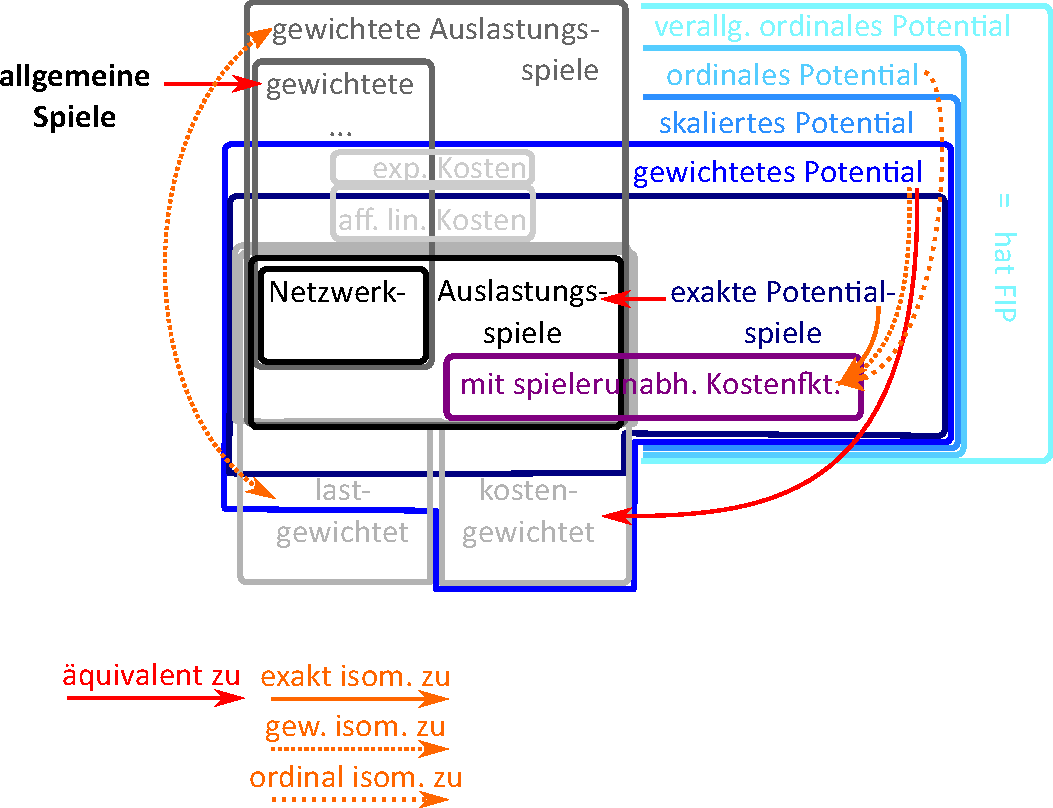
\includegraphics[width=.7\textwidth]{../Bilder/EulerDiagramm.pdf}
	\caption{Zusammenhänge zwischen den verschiedenen Spieleklassen für endliche Spiele}
\end{figure}

\phantomsection
\addcontentsline{toc}{section}{Ausblick}
\section*{Ausblick}

\todo[inline]{Ausblick schreiben}


\newpage
\nocite{*}
\printbibliography

\end{document}
